% Options for packages loaded elsewhere
\PassOptionsToPackage{unicode}{hyperref}
\PassOptionsToPackage{hyphens}{url}
%
\documentclass[
]{article}
\usepackage{amsmath,amssymb}
\usepackage{iftex}
\ifPDFTeX
  \usepackage[T1]{fontenc}
  \usepackage[utf8]{inputenc}
  \usepackage{textcomp} % provide euro and other symbols
\else % if luatex or xetex
  \usepackage{unicode-math} % this also loads fontspec
  \defaultfontfeatures{Scale=MatchLowercase}
  \defaultfontfeatures[\rmfamily]{Ligatures=TeX,Scale=1}
\fi
\usepackage{lmodern}
\ifPDFTeX\else
  % xetex/luatex font selection
\fi
% Use upquote if available, for straight quotes in verbatim environments
\IfFileExists{upquote.sty}{\usepackage{upquote}}{}
\IfFileExists{microtype.sty}{% use microtype if available
  \usepackage[]{microtype}
  \UseMicrotypeSet[protrusion]{basicmath} % disable protrusion for tt fonts
}{}
\makeatletter
\@ifundefined{KOMAClassName}{% if non-KOMA class
  \IfFileExists{parskip.sty}{%
    \usepackage{parskip}
  }{% else
    \setlength{\parindent}{0pt}
    \setlength{\parskip}{6pt plus 2pt minus 1pt}}
}{% if KOMA class
  \KOMAoptions{parskip=half}}
\makeatother
\usepackage{xcolor}
\usepackage[margin=1in]{geometry}
\usepackage{graphicx}
\makeatletter
\def\maxwidth{\ifdim\Gin@nat@width>\linewidth\linewidth\else\Gin@nat@width\fi}
\def\maxheight{\ifdim\Gin@nat@height>\textheight\textheight\else\Gin@nat@height\fi}
\makeatother
% Scale images if necessary, so that they will not overflow the page
% margins by default, and it is still possible to overwrite the defaults
% using explicit options in \includegraphics[width, height, ...]{}
\setkeys{Gin}{width=\maxwidth,height=\maxheight,keepaspectratio}
% Set default figure placement to htbp
\makeatletter
\def\fps@figure{htbp}
\makeatother
\setlength{\emergencystretch}{3em} % prevent overfull lines
\providecommand{\tightlist}{%
  \setlength{\itemsep}{0pt}\setlength{\parskip}{0pt}}
\setcounter{secnumdepth}{-\maxdimen} % remove section numbering
\ifLuaTeX
  \usepackage{selnolig}  % disable illegal ligatures
\fi
\usepackage{bookmark}
\IfFileExists{xurl.sty}{\usepackage{xurl}}{} % add URL line breaks if available
\urlstyle{same}
\hypersetup{
  pdftitle={When Do Discounts Matter?},
  pdfauthor={Tanetpong (Ned) Choungprayoon},
  hidelinks,
  pdfcreator={LaTeX via pandoc}}

\title{When Do Discounts Matter?}
\author{Tanetpong (Ned) Choungprayoon}
\date{}

\begin{document}
\maketitle

\section{\centering Project Summary}

Most quantitative research papers model the effect of price promotions
as the effect of changes in the final retail price while consumer
behavior research suggests the potential framing phenomena in which
customers can evaluate retail price and discounts differently. By taking
this behavioral assumption in the sales-response model, we can estimate
the discounts' elasticities apart from price elasticities and
investigate its systematic drivers from brand factors, category factors
and store formats using second-stage regression. Using replicable
simulated data (as I cannot share an actual data), I attempted to show
that discounts are not equally effective across brands, categories and
store format and I can estimate their differential effects.

\section{\centering Table of Contents}

\begin{itemize}
\tightlist
\item
  Model-Free Evidence:

  \begin{itemize}
  \tightlist
  \item
    Data explonatory analysis of plausible relationship between brands'
    sales and discounts across store formats
  \end{itemize}
\item
  First-Stage Analysis:

  \begin{itemize}
  \tightlist
  \item
    Estimated discounts elasticity for each brand
  \end{itemize}
\item
  Second-Stage Analysis:

  \begin{itemize}
  \tightlist
  \item
    Estimated determinants of store format and brand characteristics on
    discounts elasticity
  \end{itemize}
\end{itemize}

\newpage

\section{Model-Free Evidence}

\begin{itemize}
\tightlist
\item
  We explore relationship between brands' sales and offered discounts by
  simple plotting.
\end{itemize}

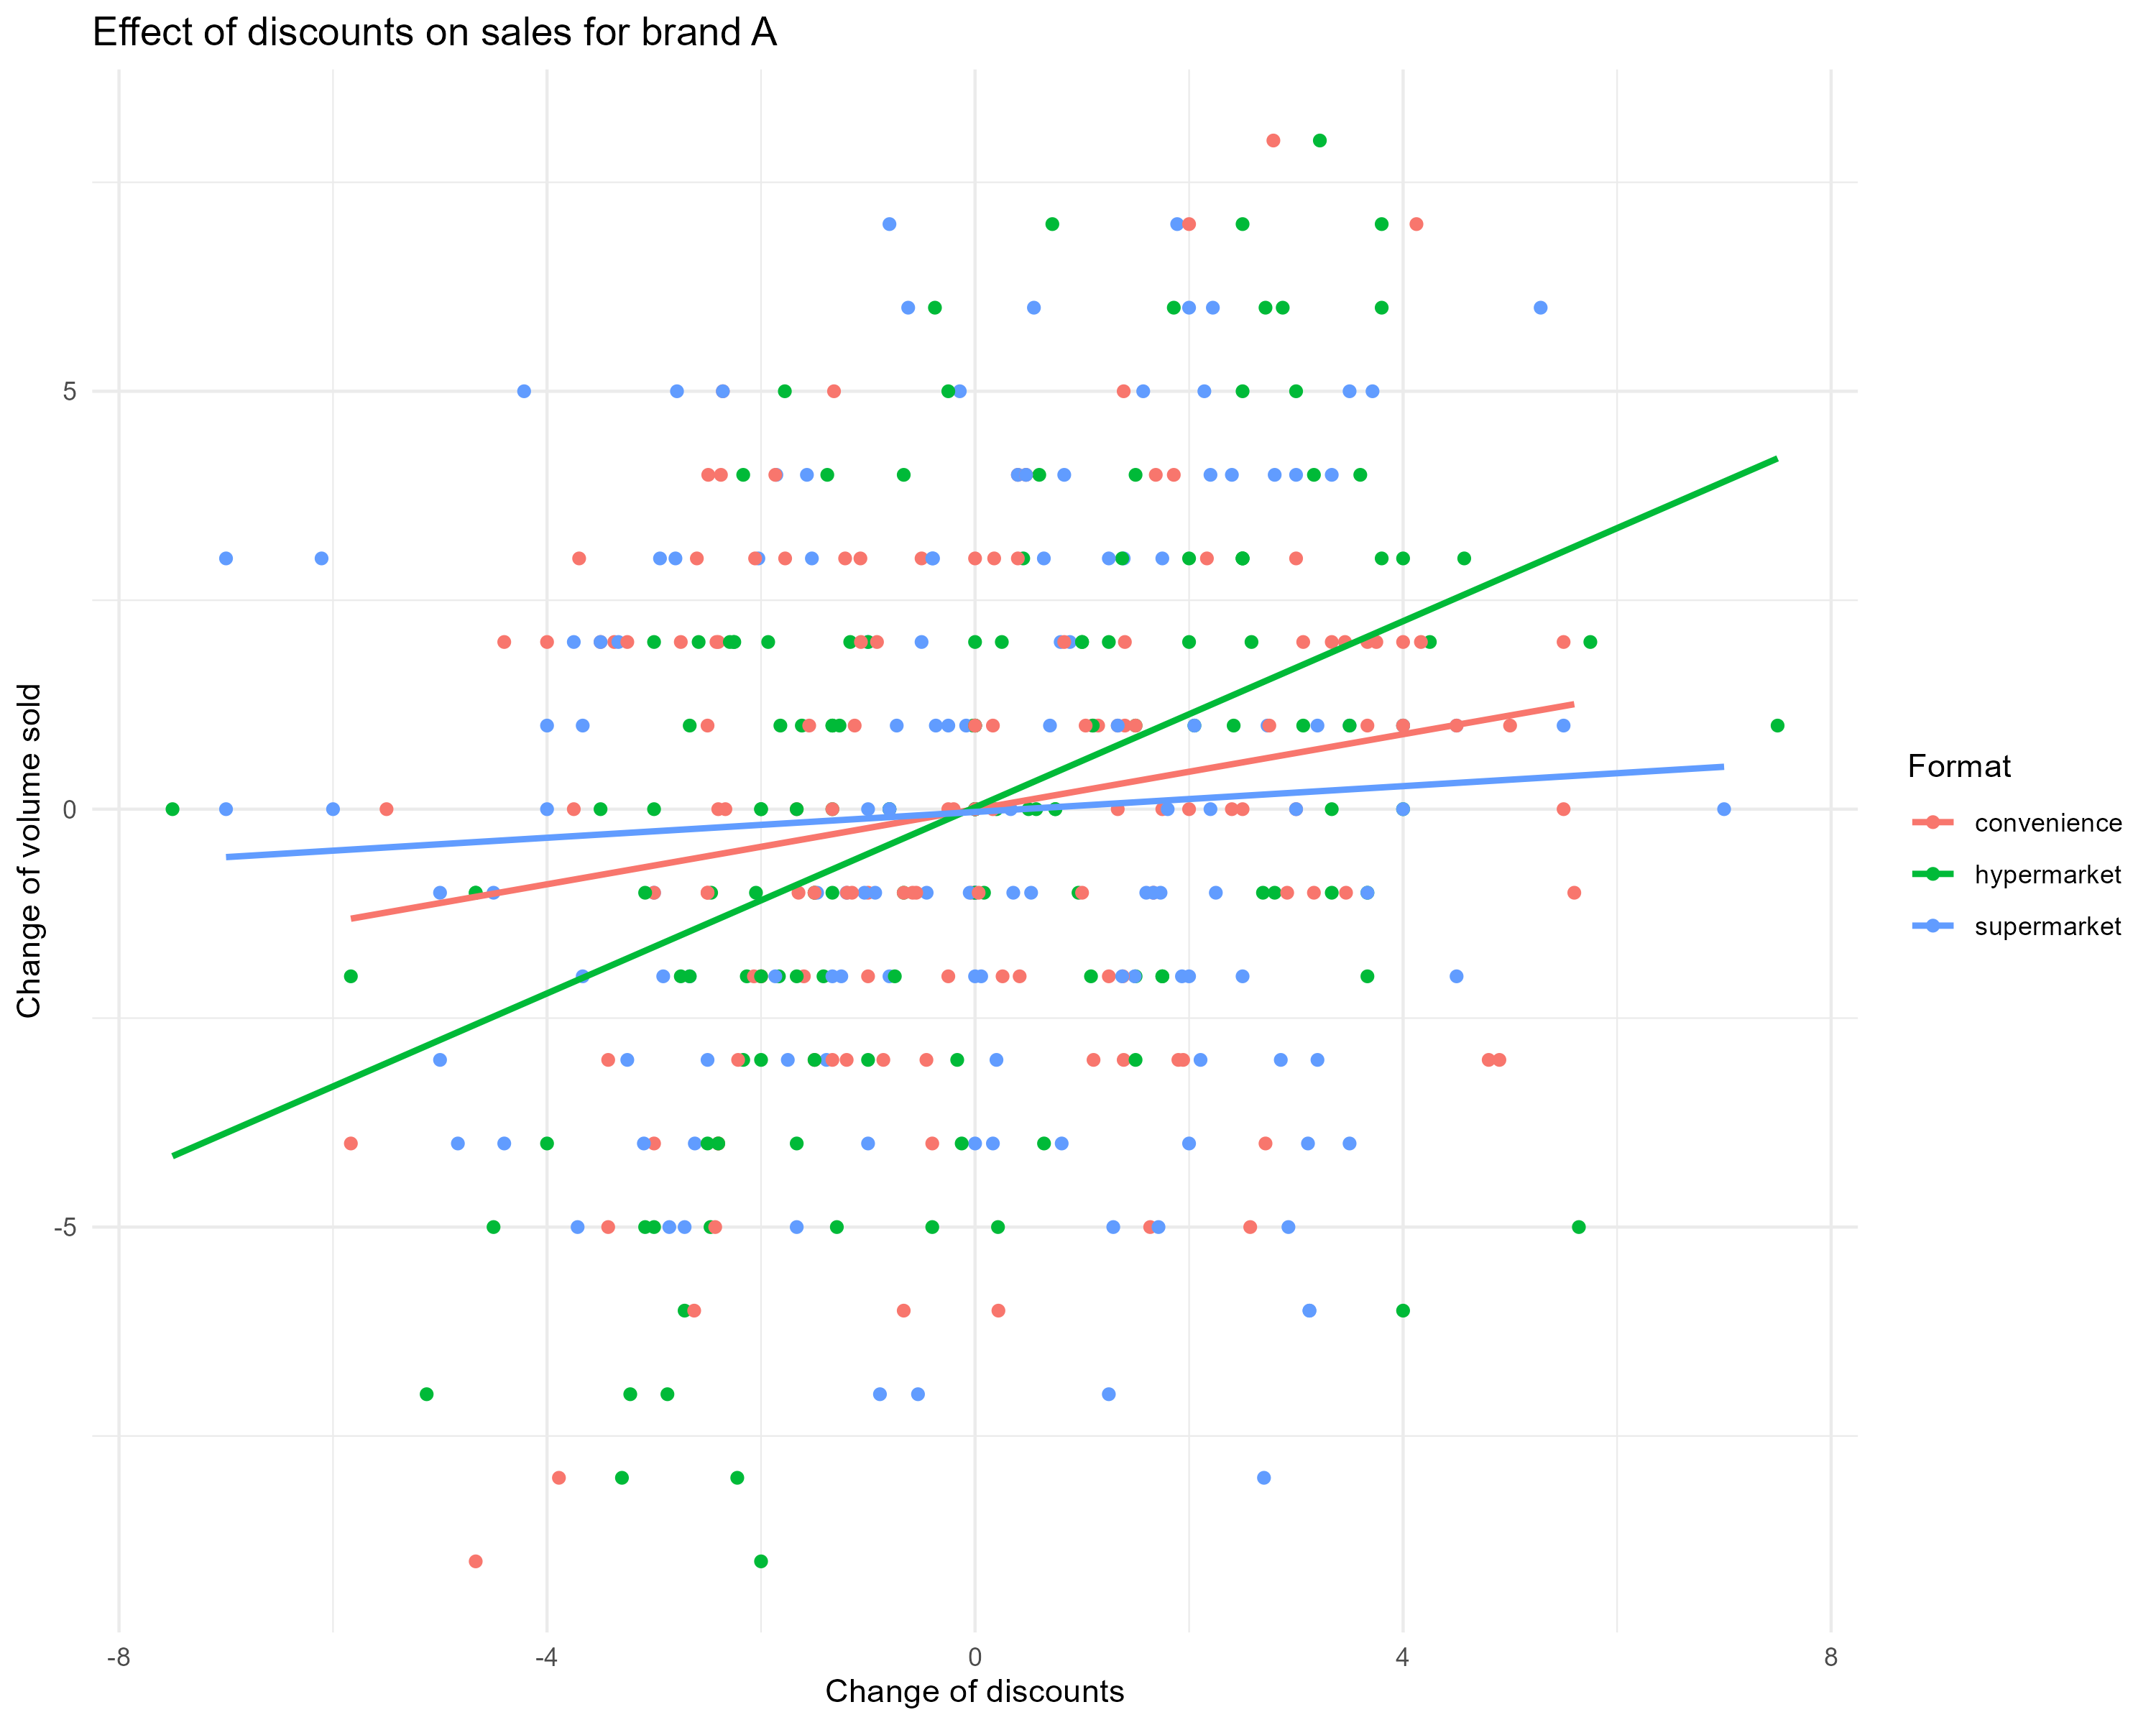
\includegraphics{../../gen/audit/discounts_sales_brand_a.png}
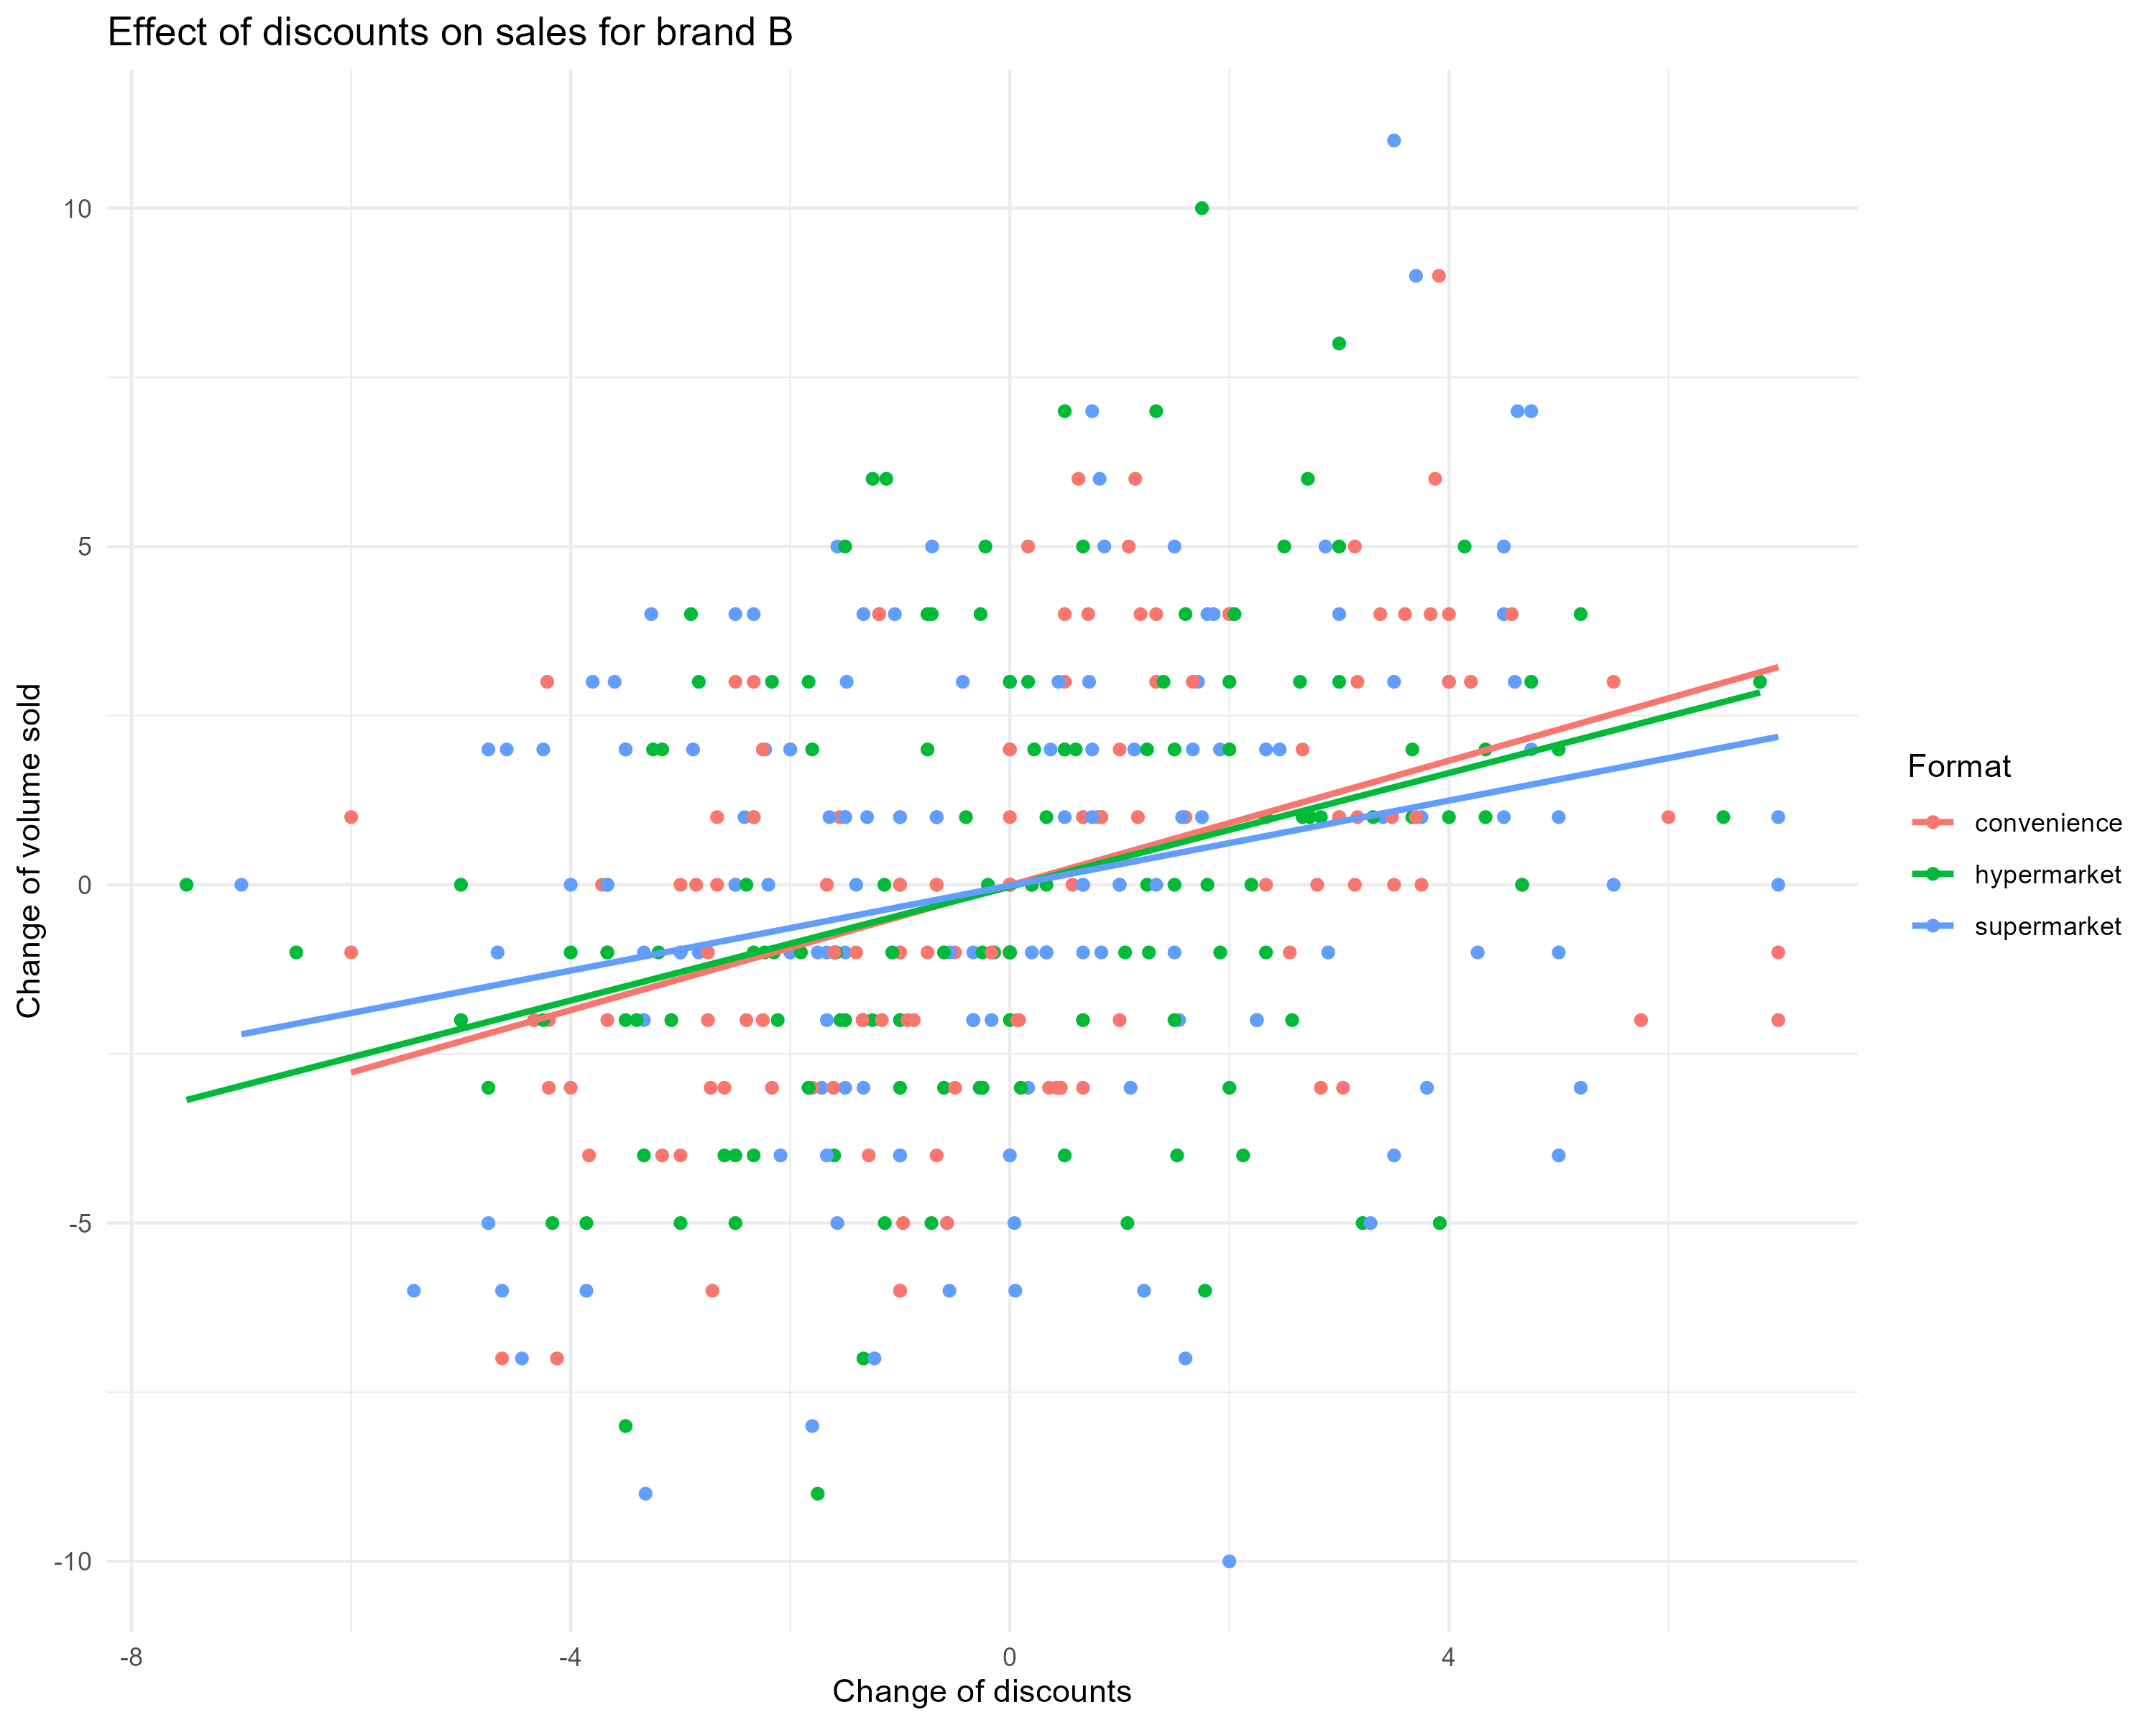
\includegraphics{../../gen/audit/discounts_sales_brand_b.png}
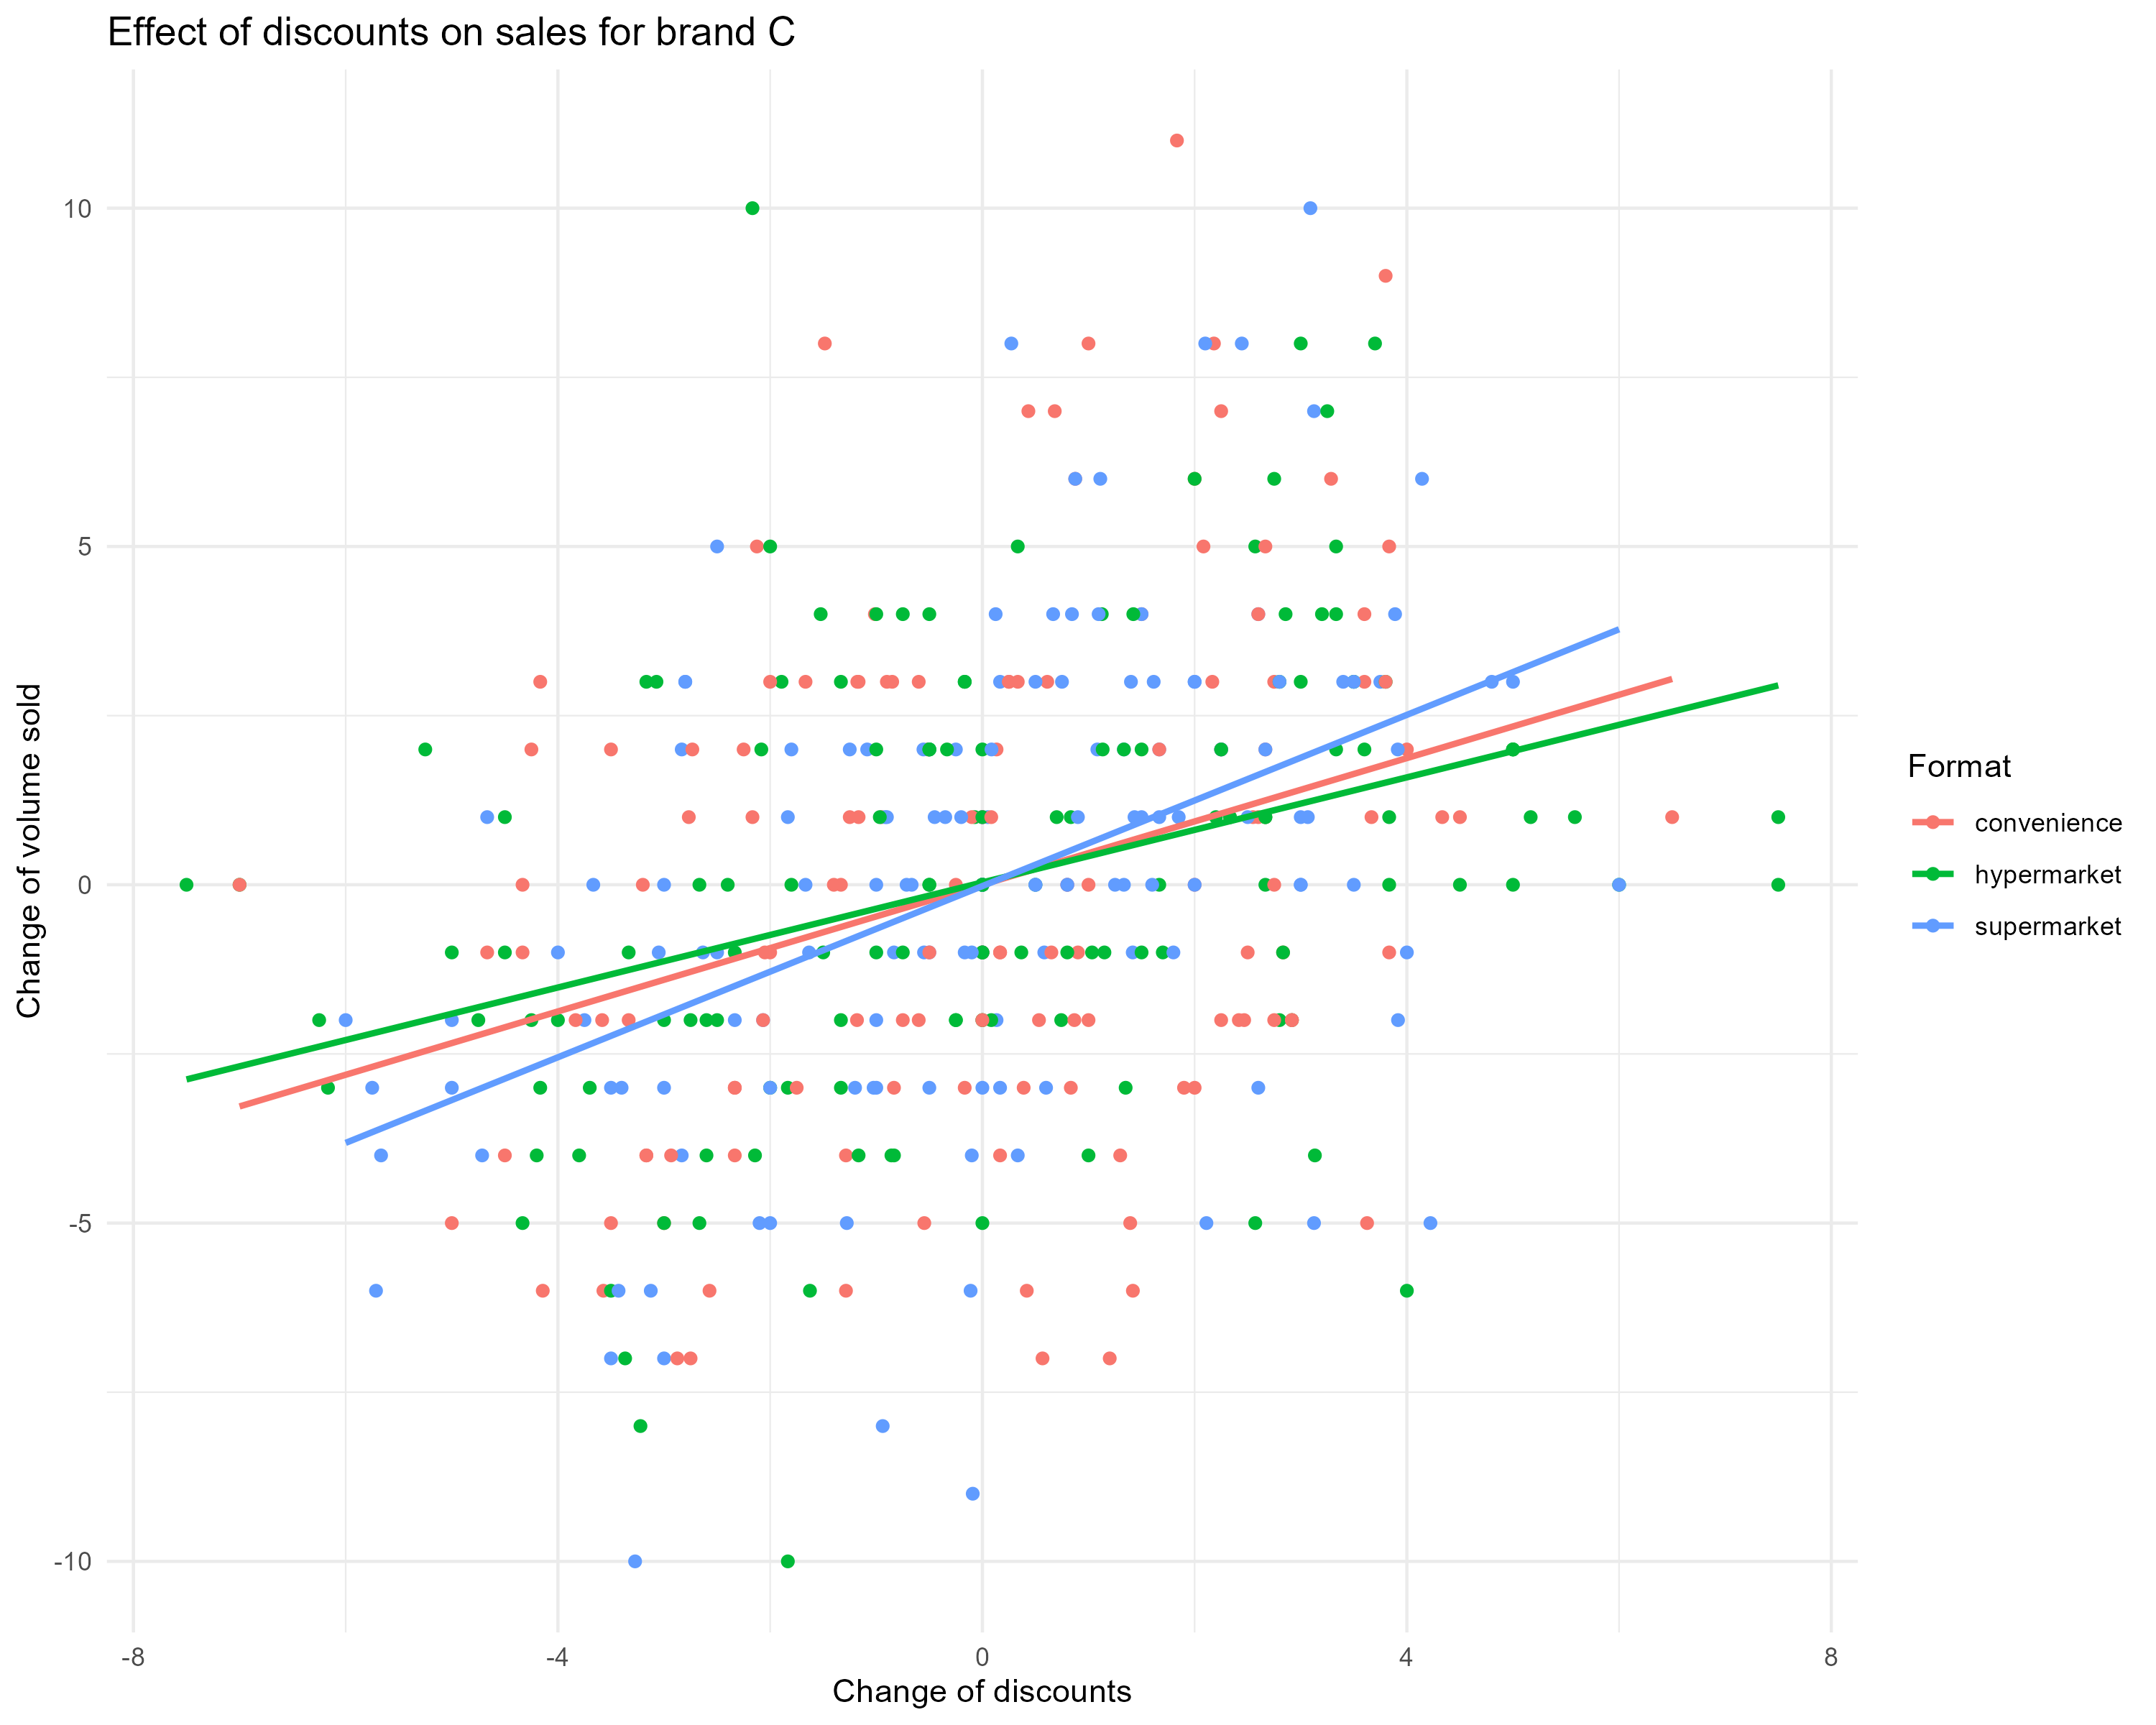
\includegraphics{../../gen/audit/discounts_sales_brand_c.png}
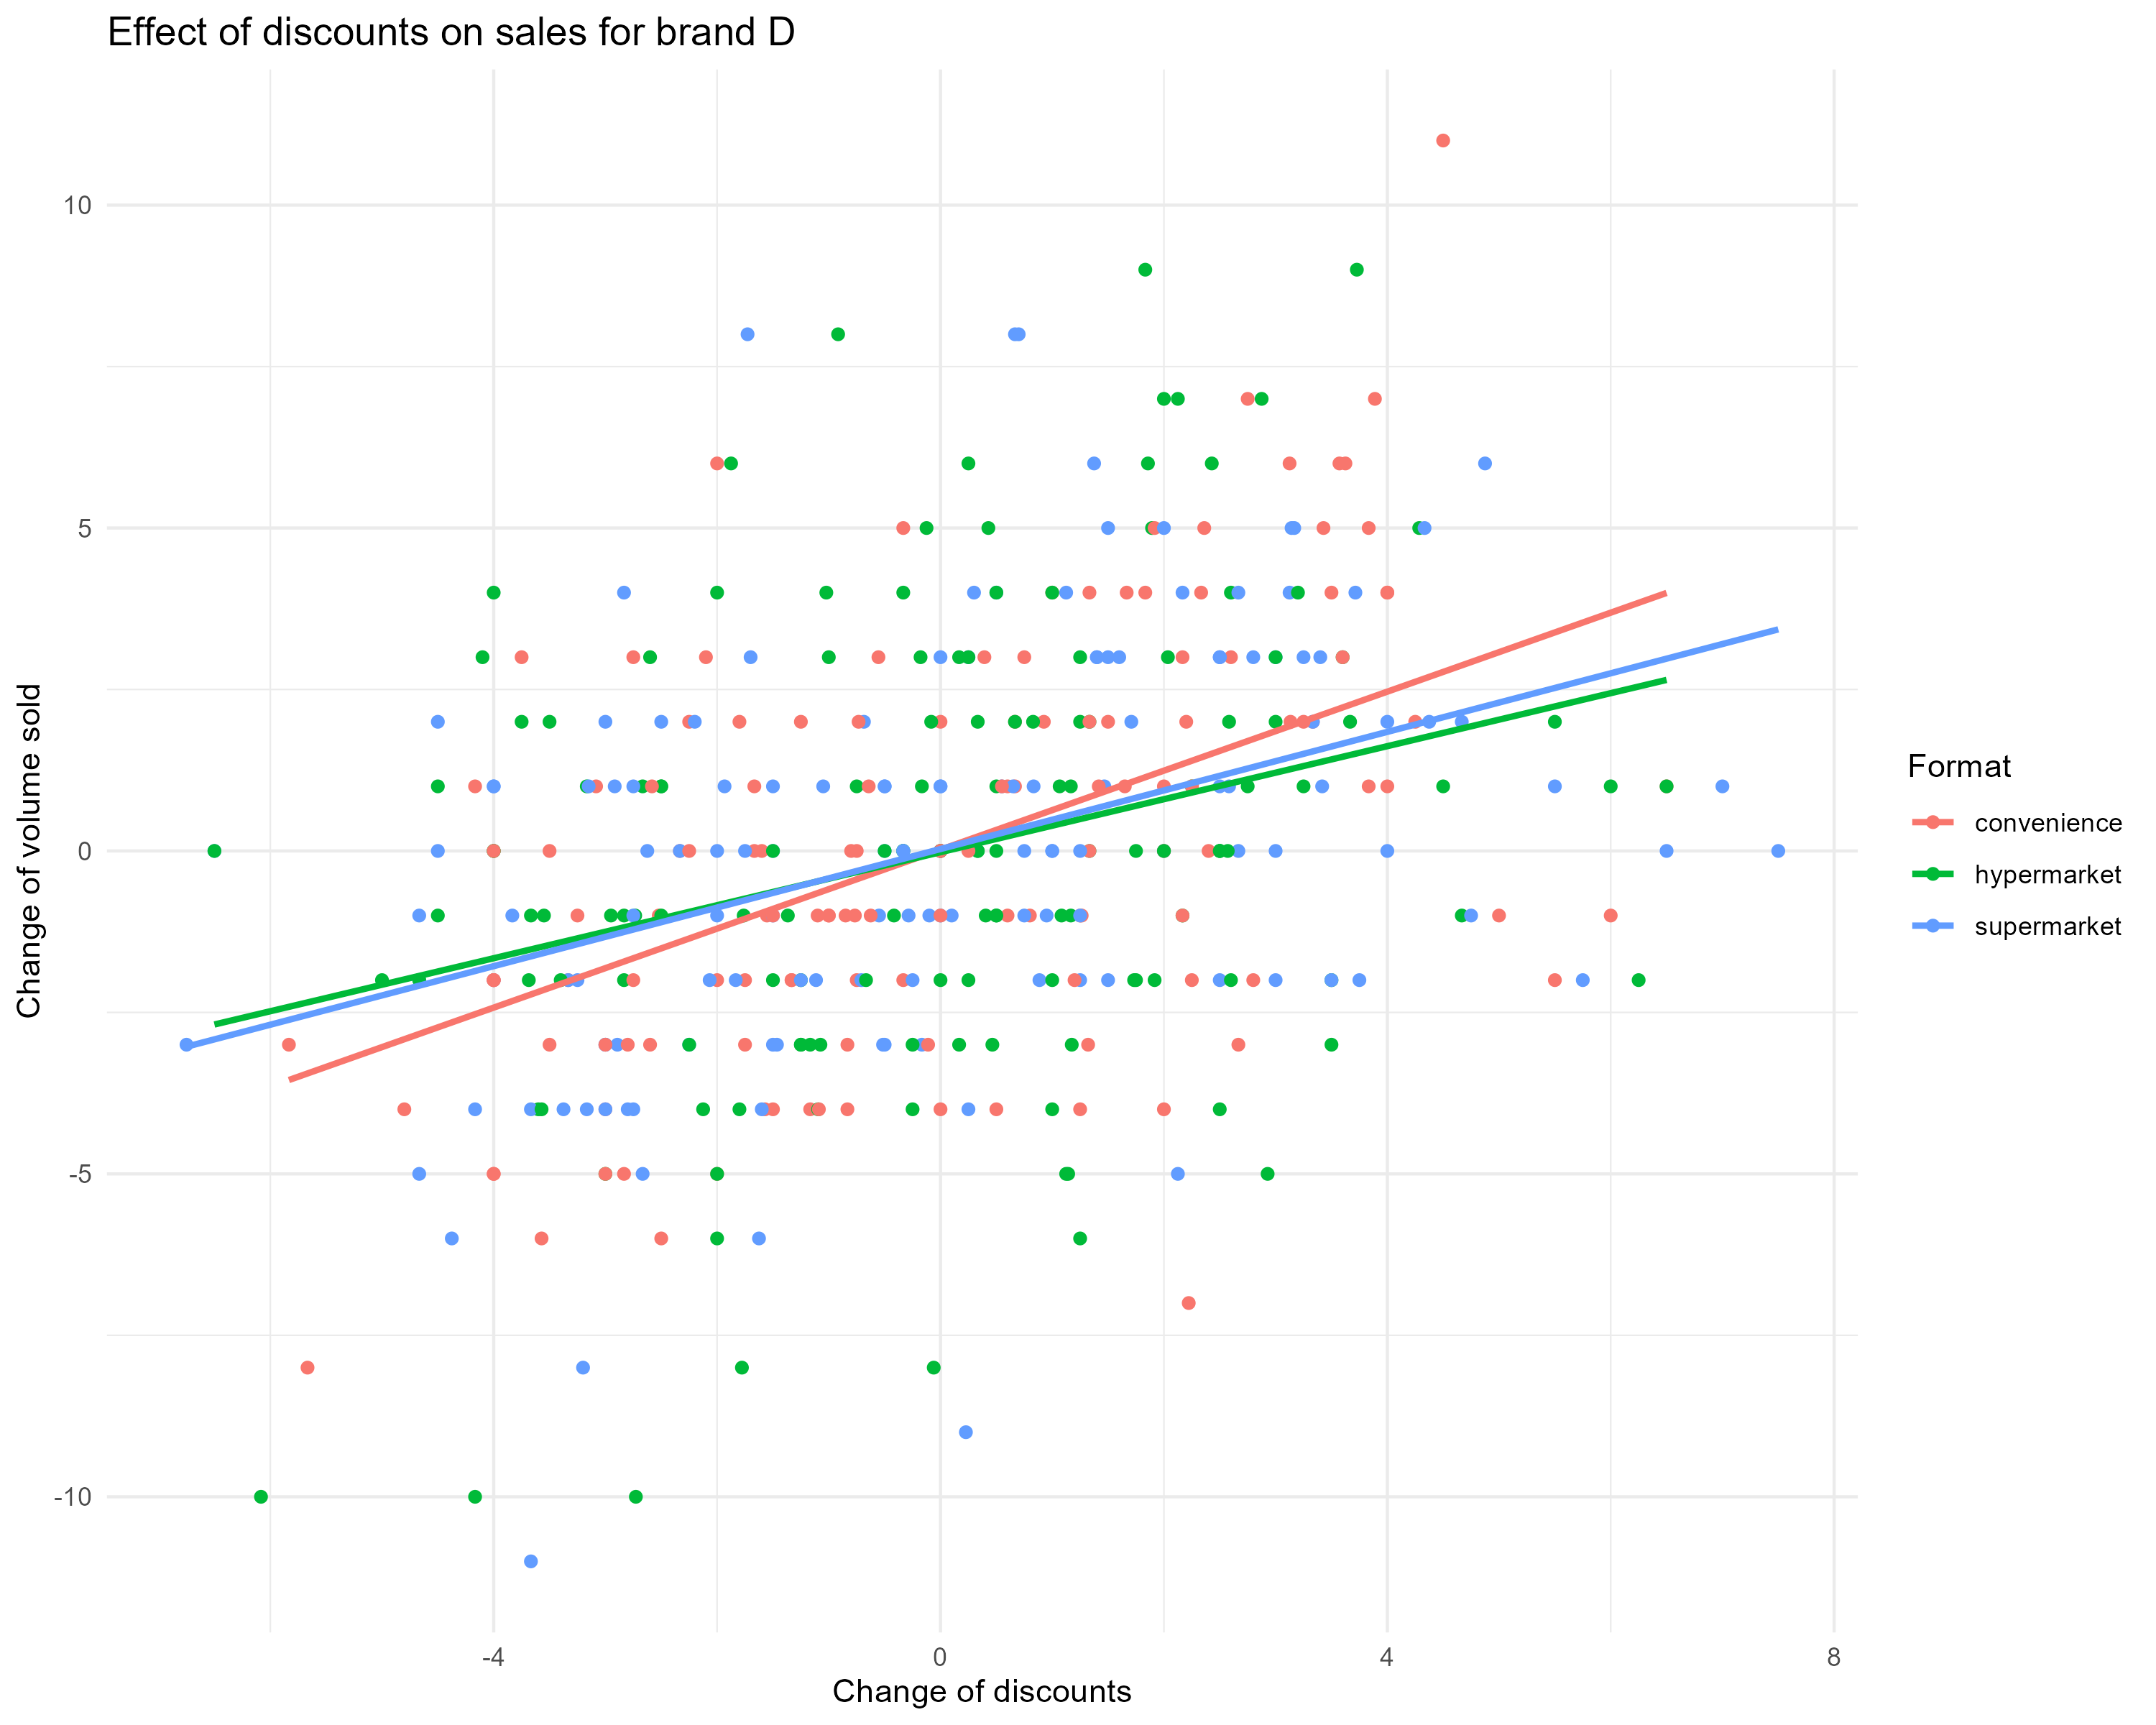
\includegraphics{../../gen/audit/discounts_sales_brand_d.png}
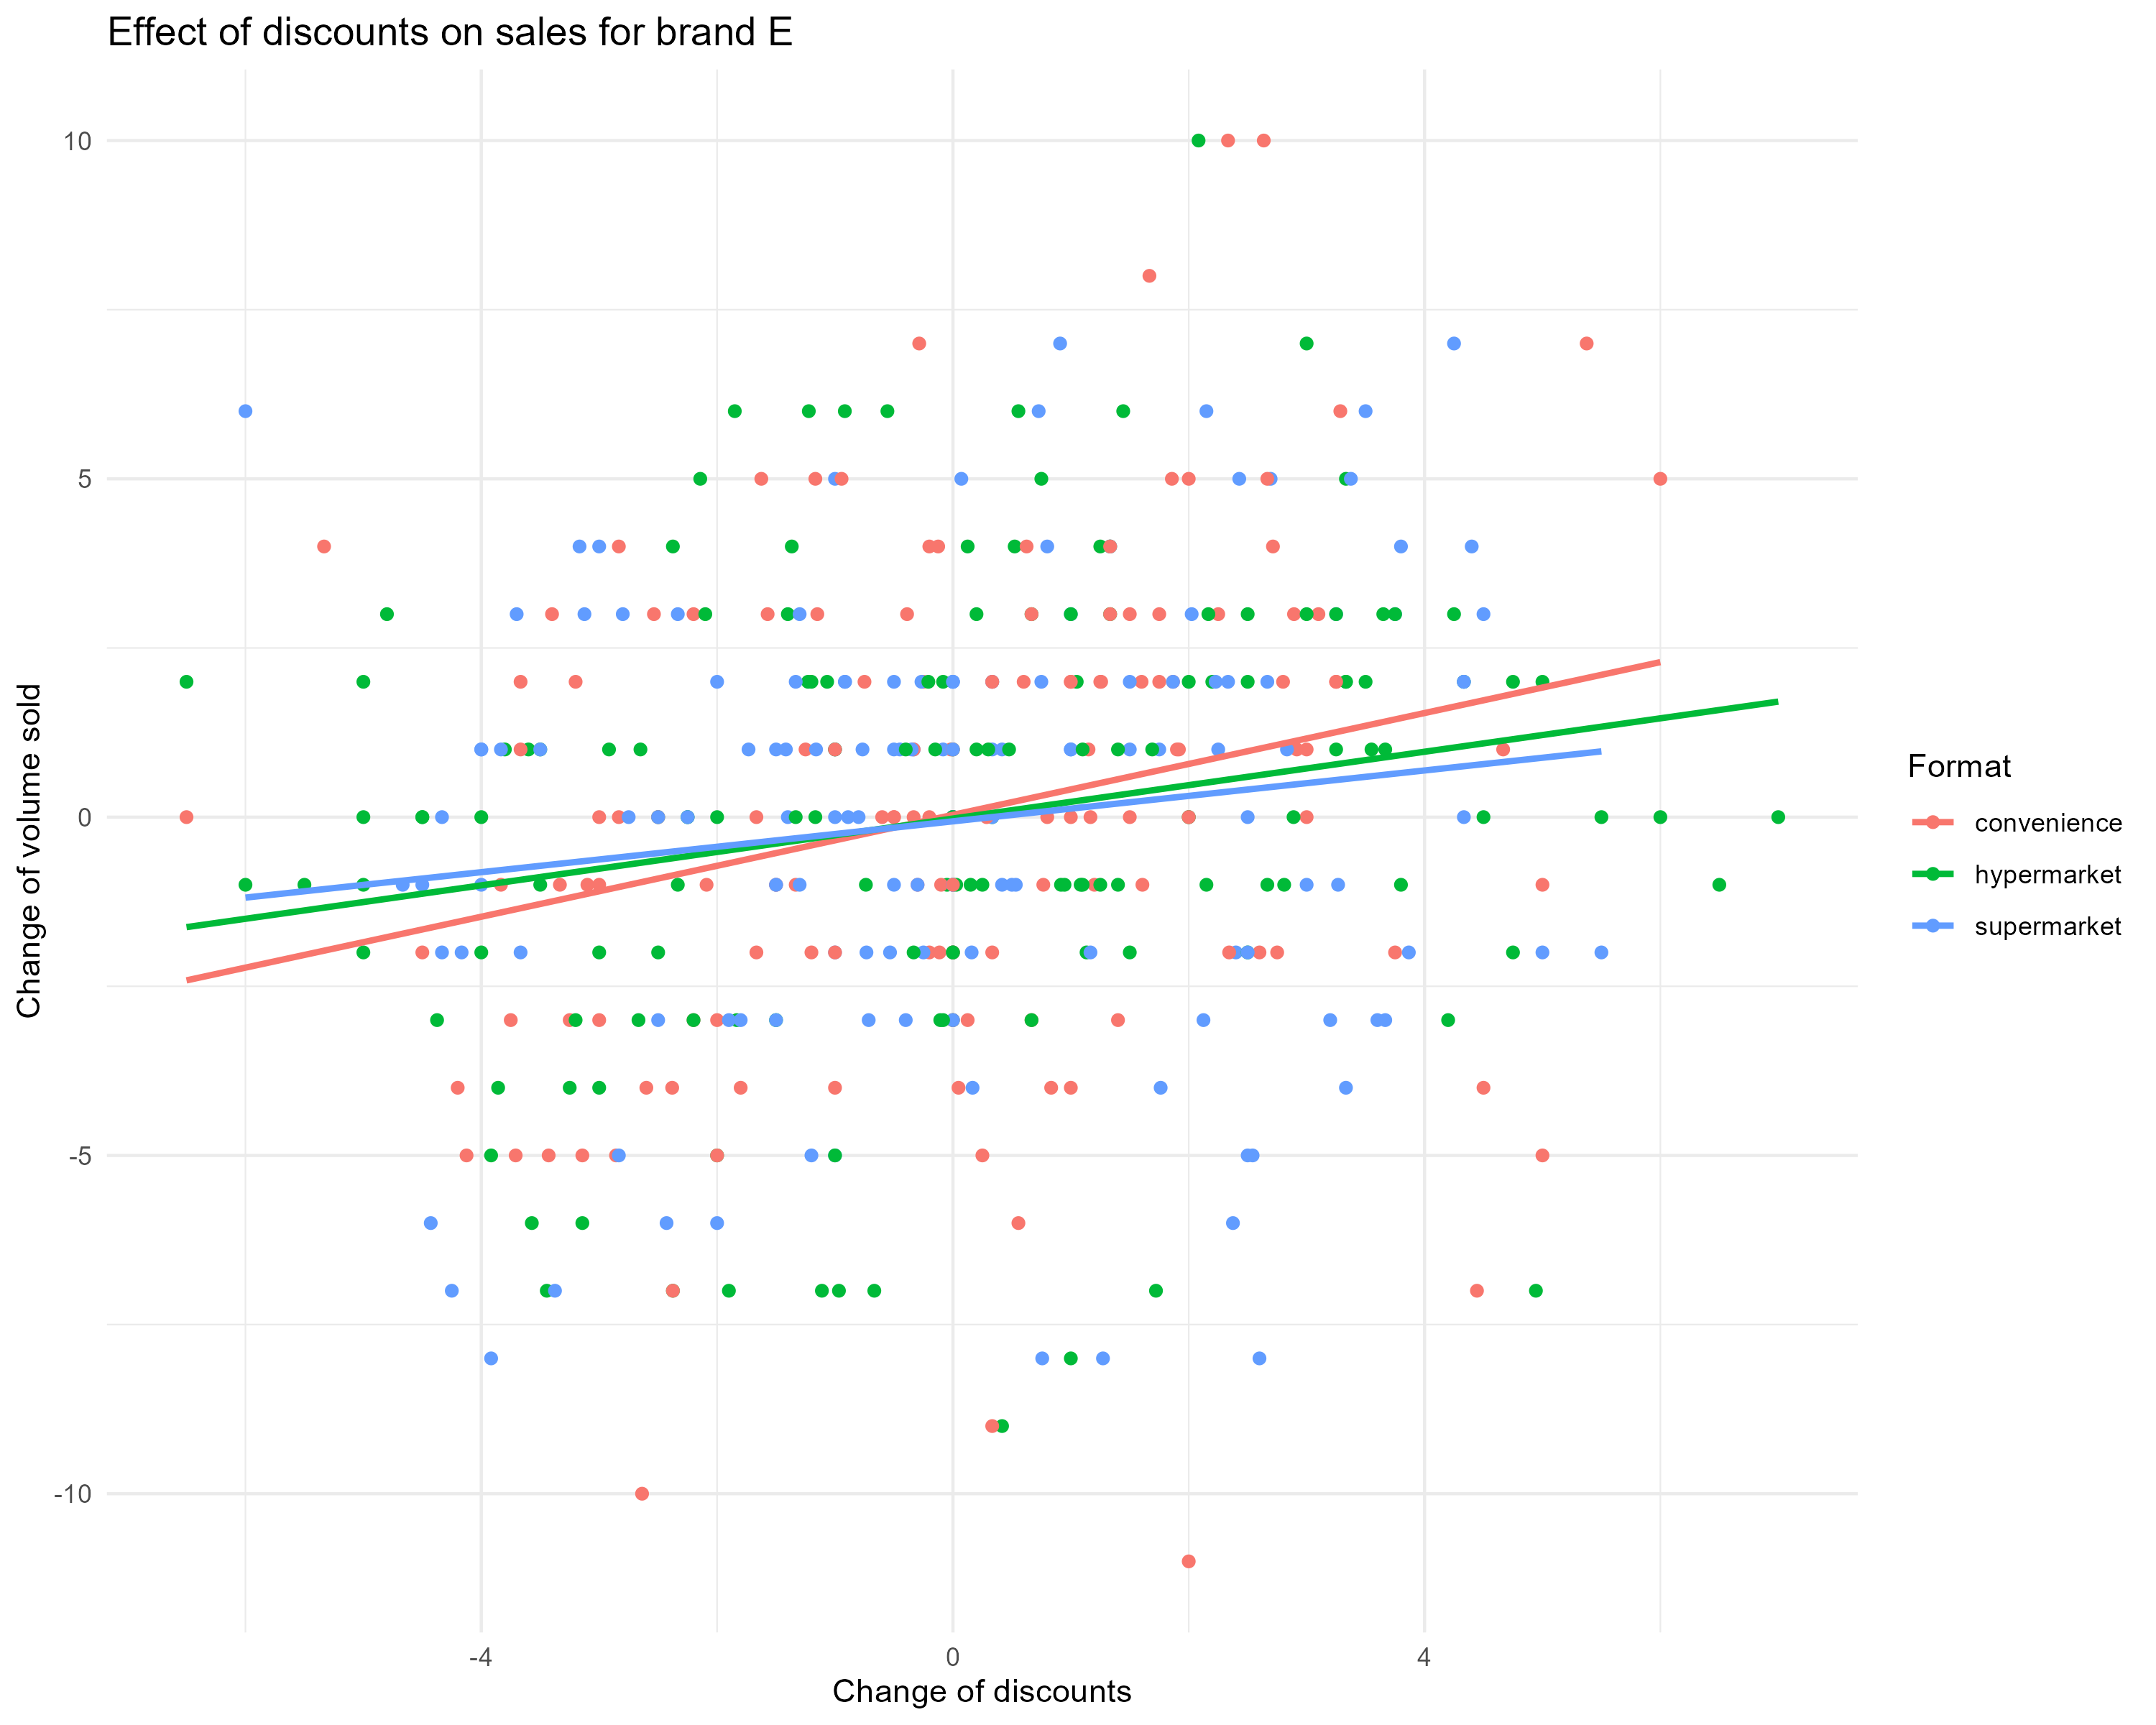
\includegraphics{../../gen/audit/discounts_sales_brand_e.png}

\begin{itemize}
\tightlist
\item
  We further plot the relationship between brands' sales and offered
  discounts across different store formats (i.e., hypermarket,
  supermarket and convenience store)
\end{itemize}

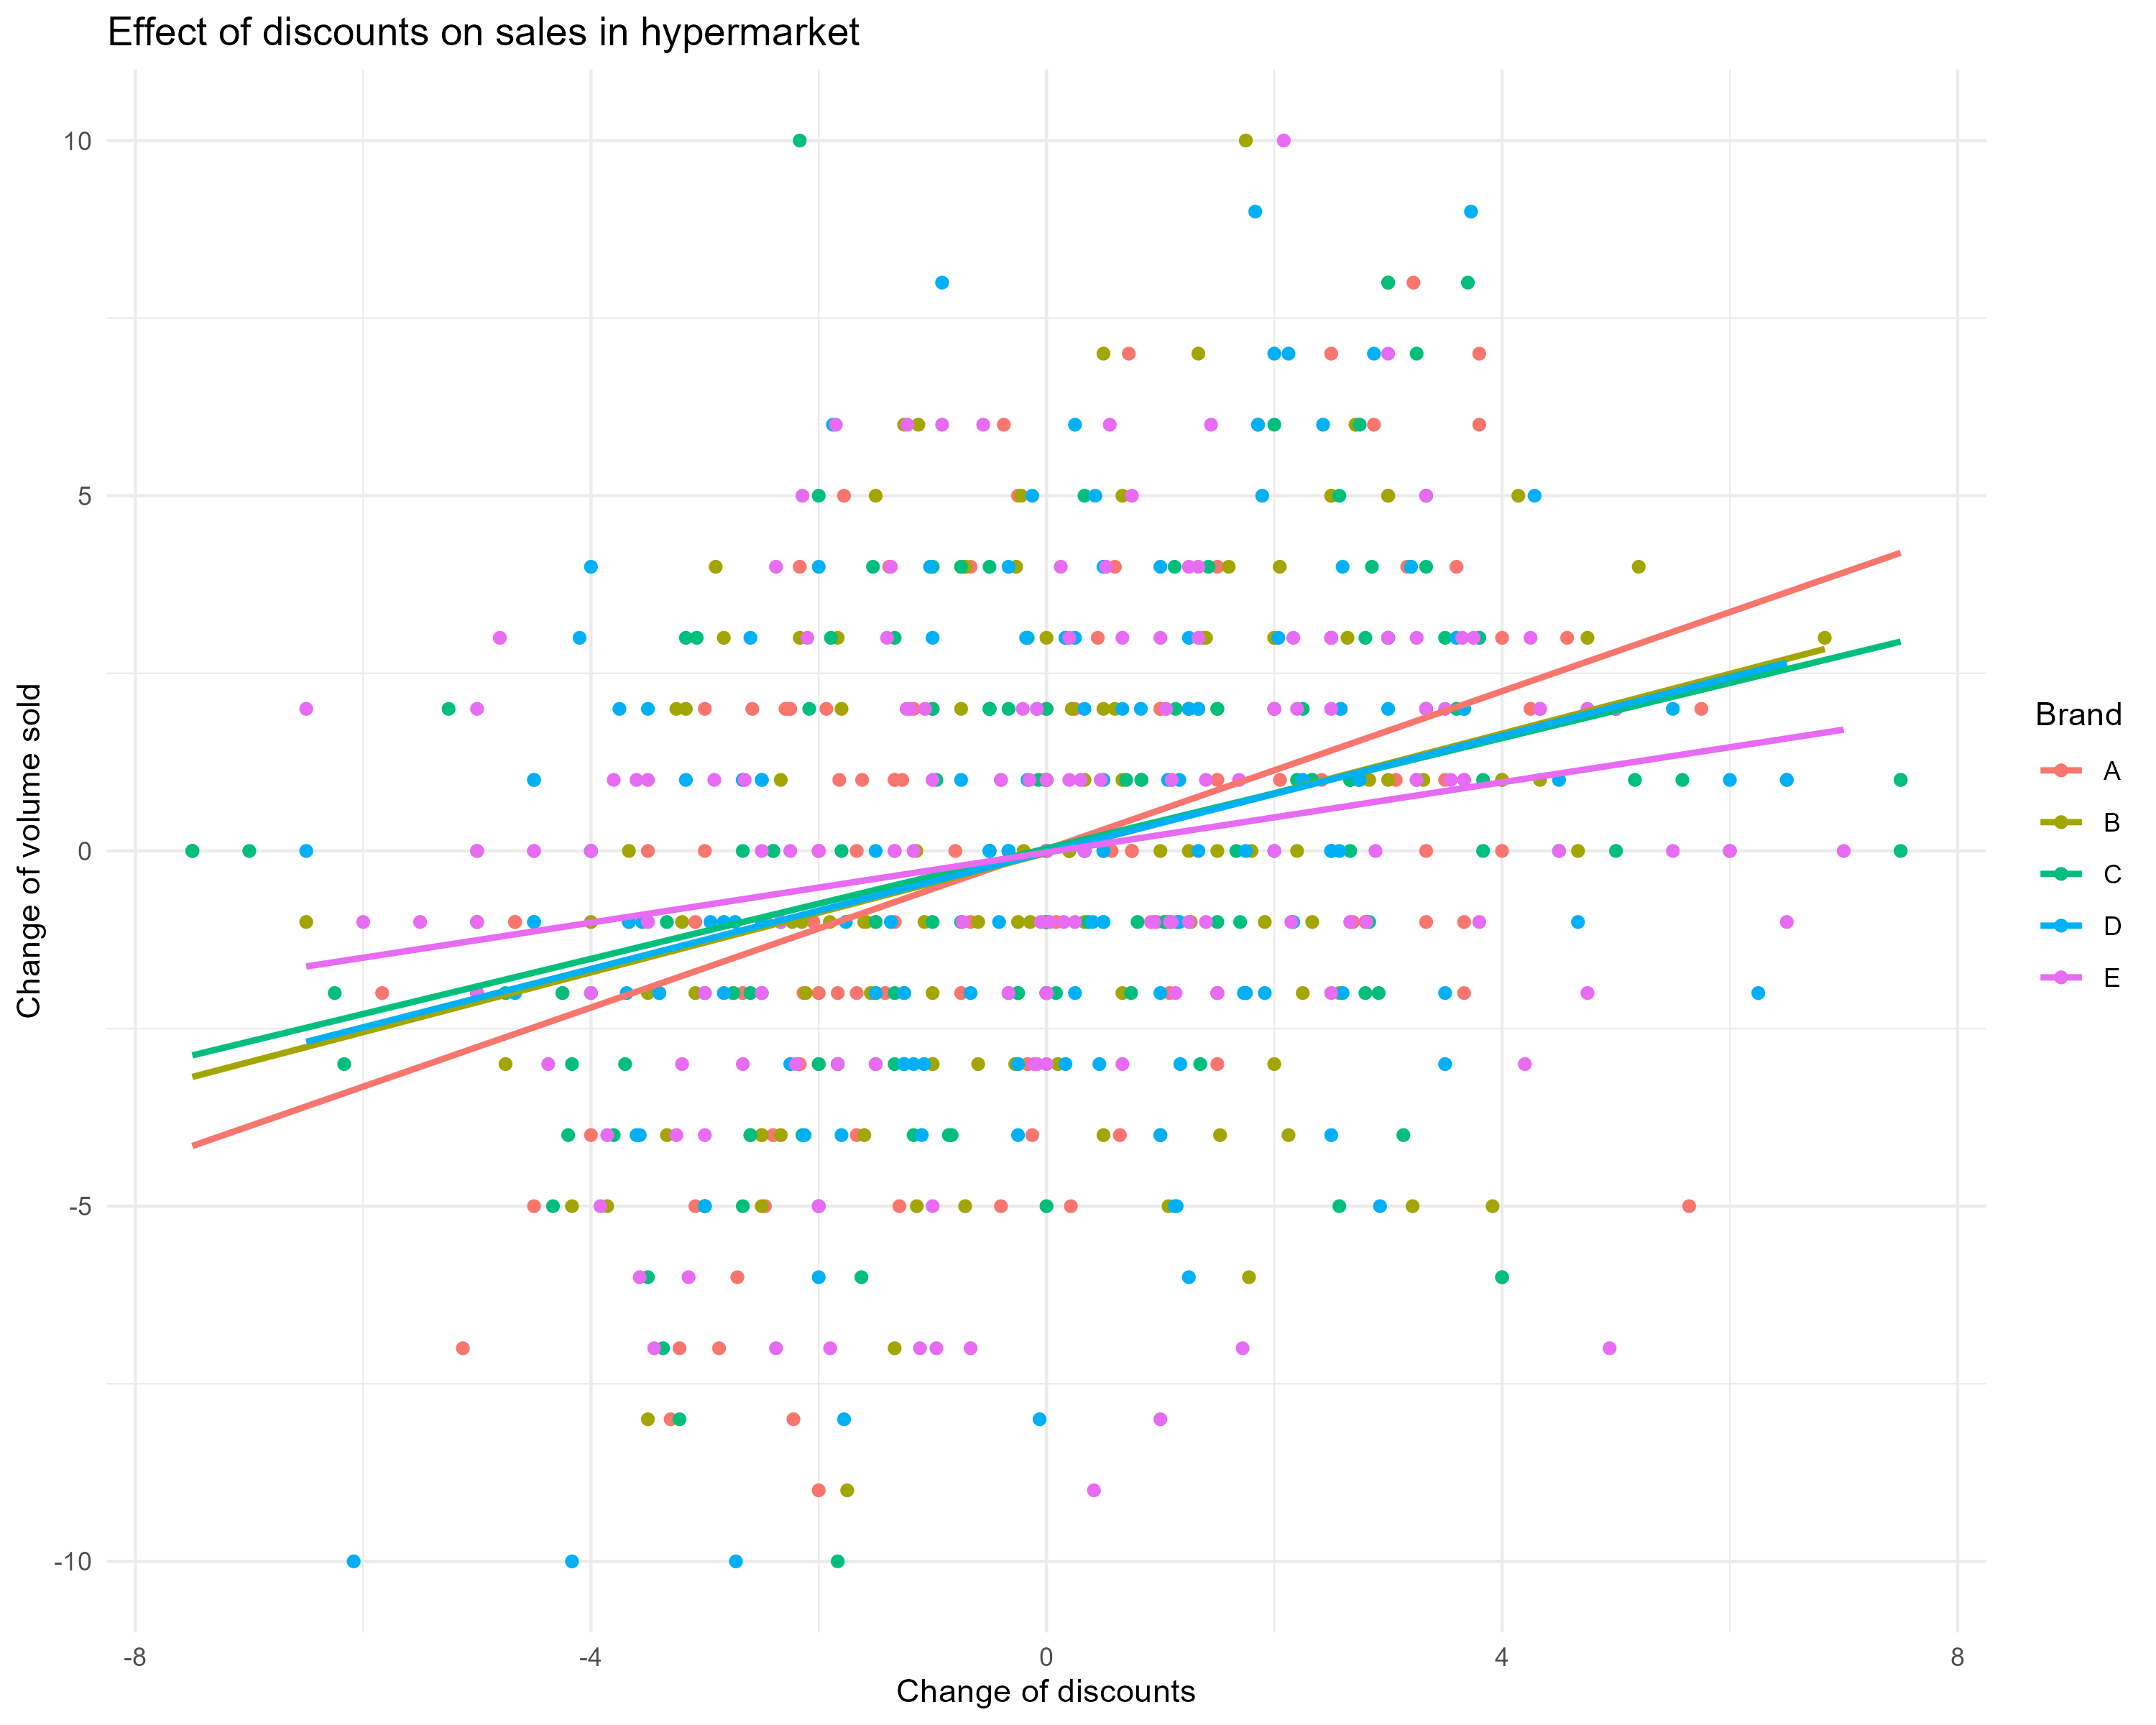
\includegraphics{../../gen/audit/discounts_sales_in_hypermarket.png}
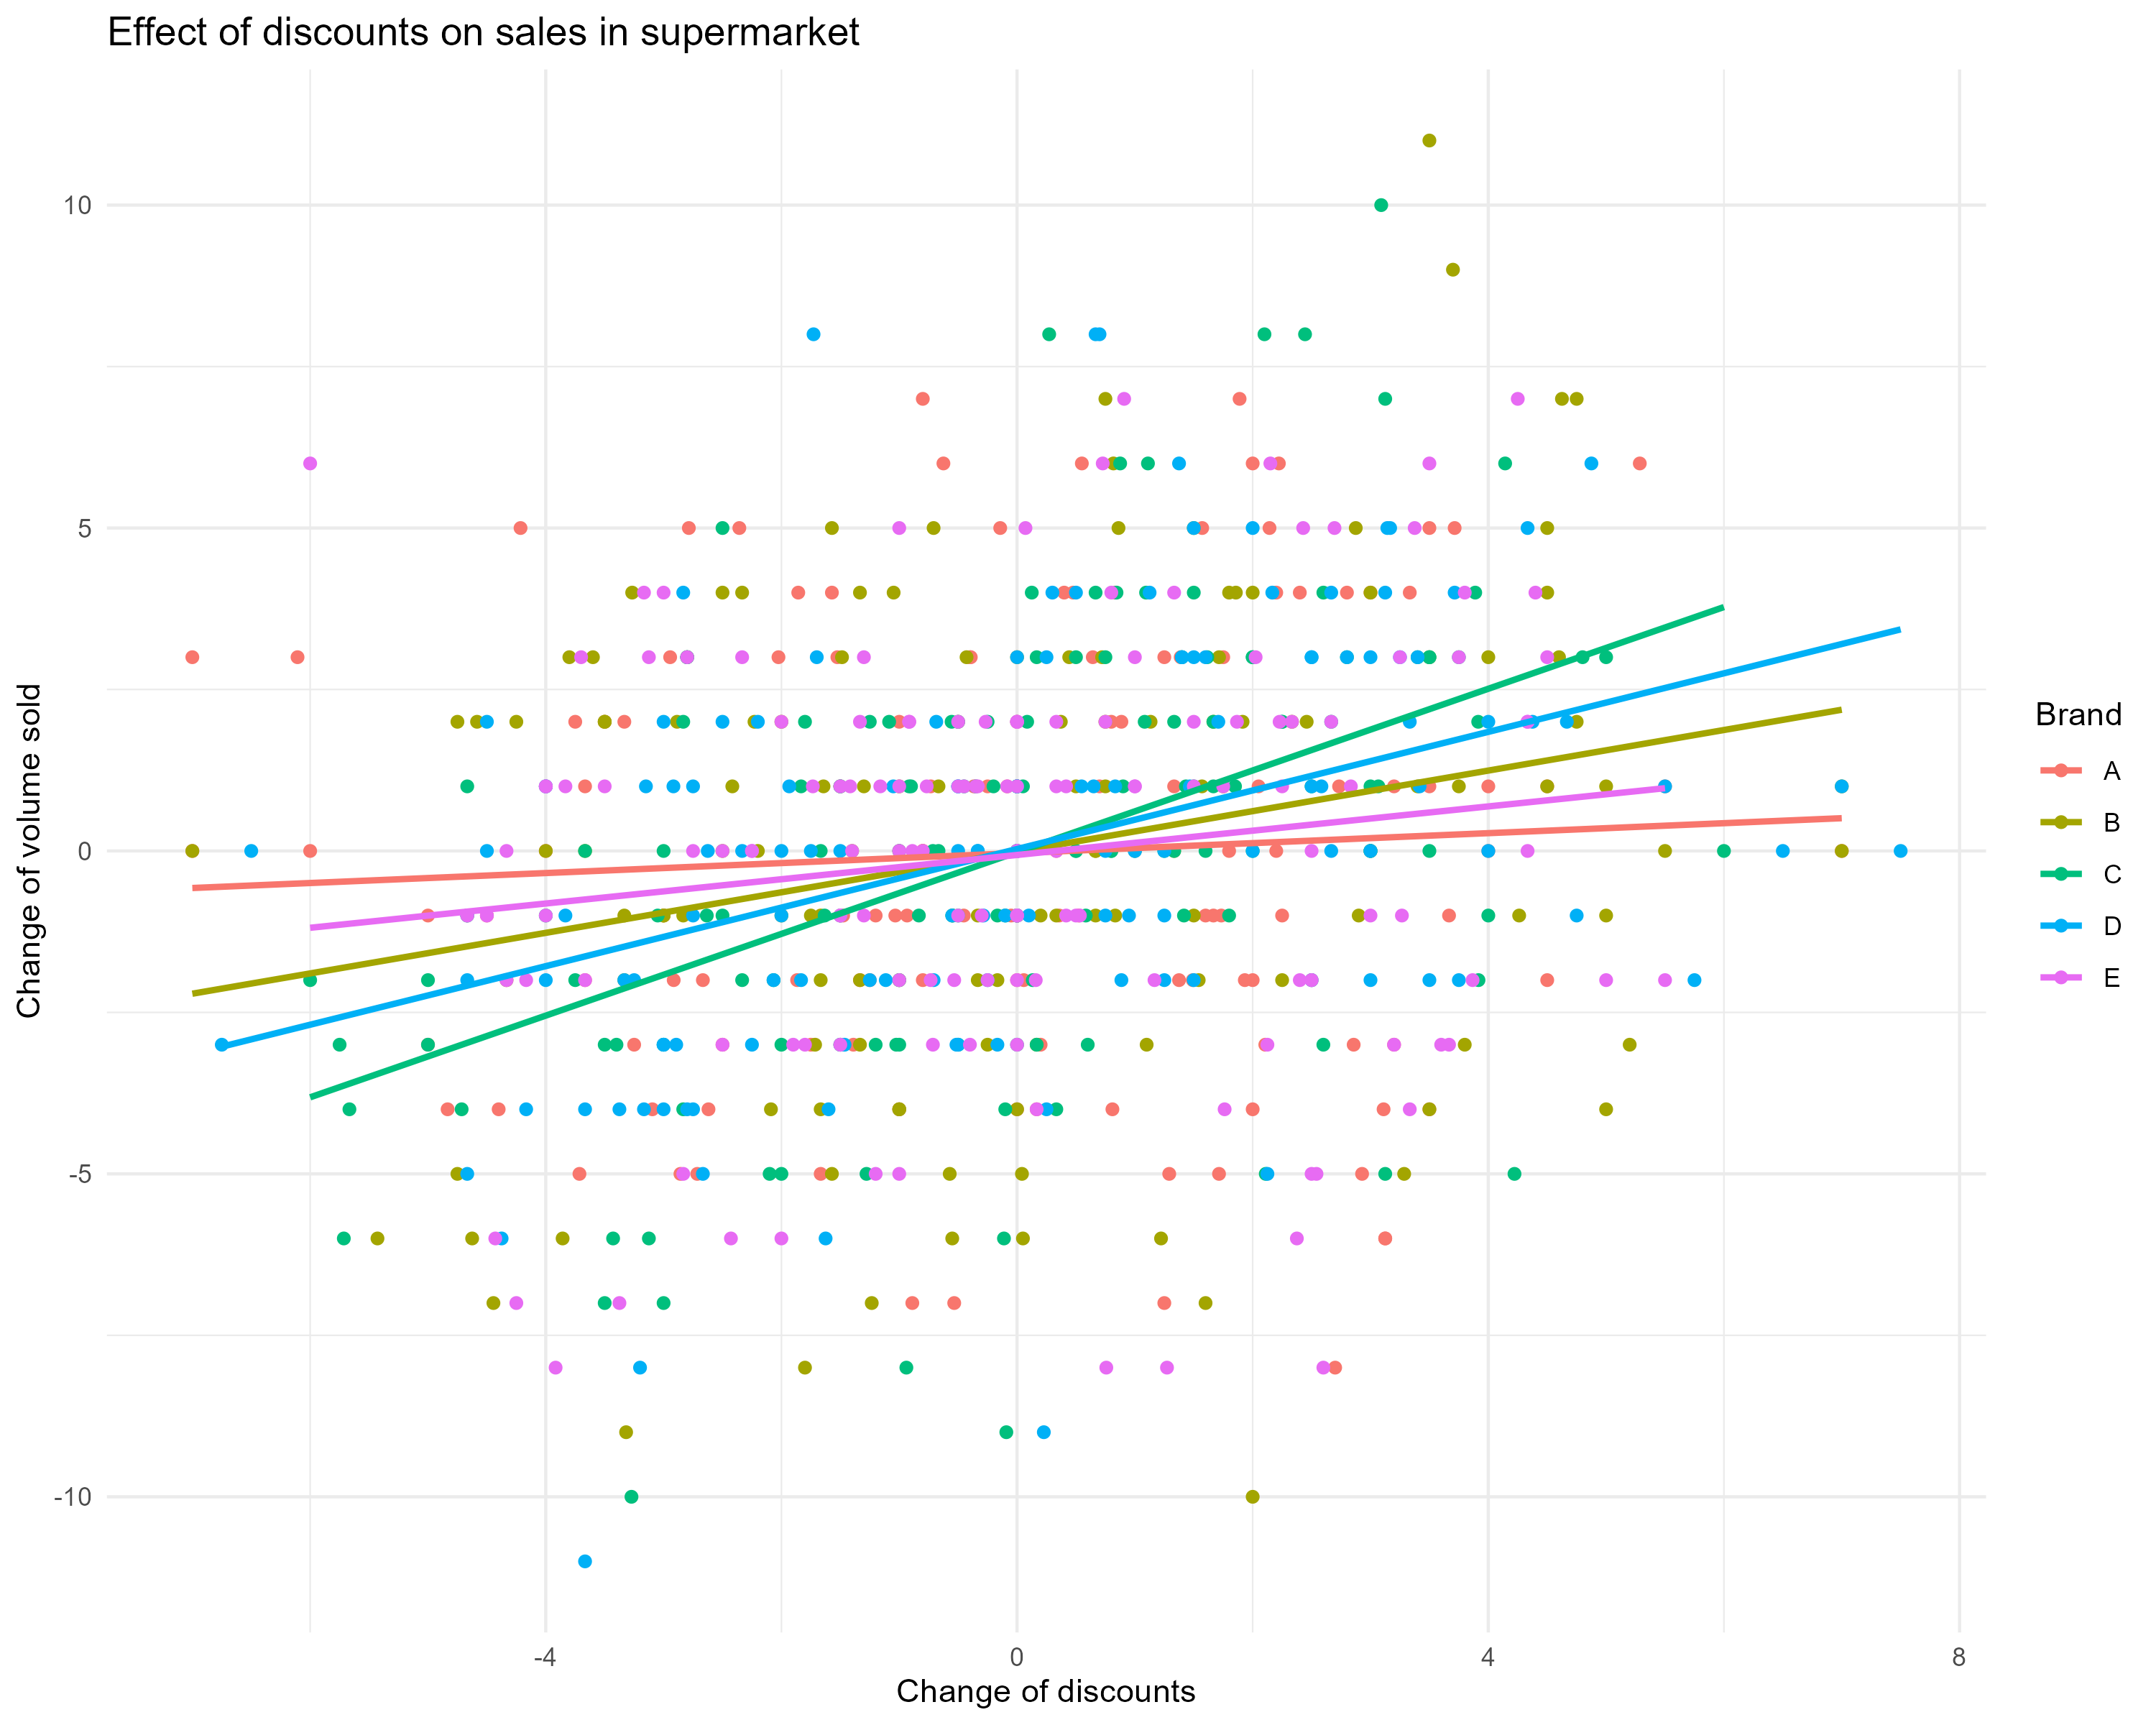
\includegraphics{../../gen/audit/discounts_sales_in_supermarket.png}

\begin{figure}
\centering
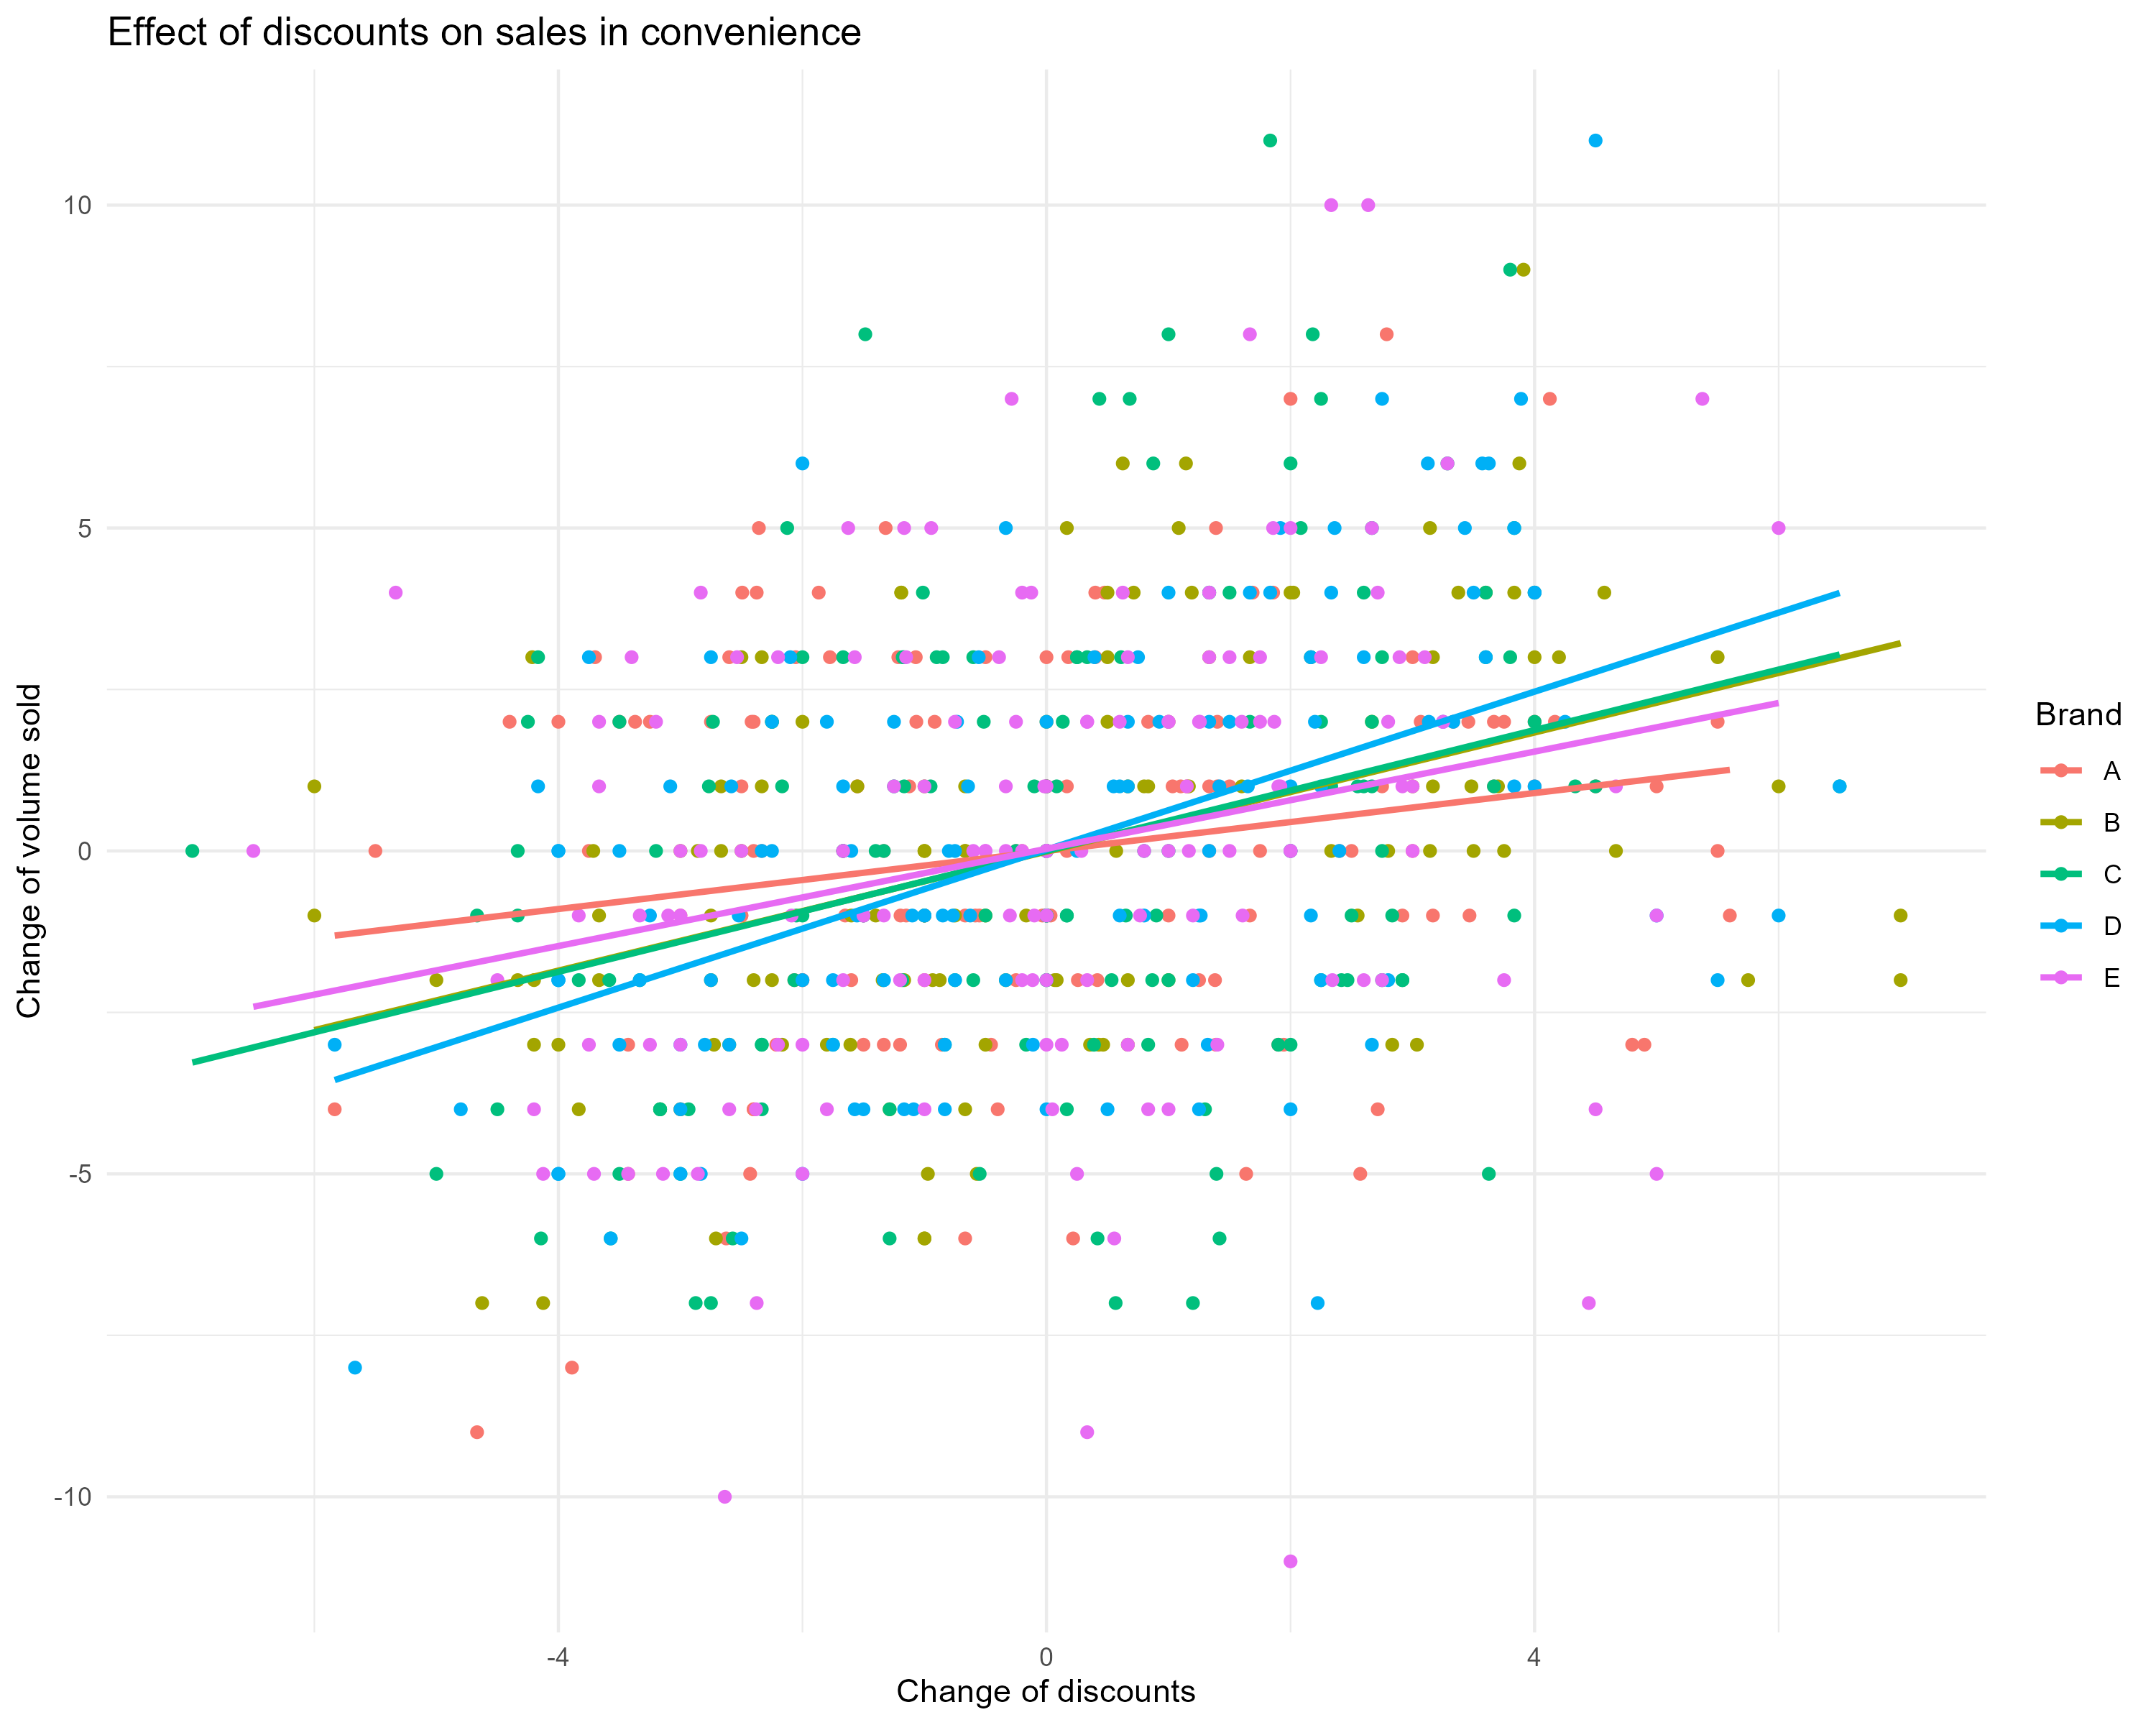
\includegraphics{../../gen/audit/discounts_sales_in_convenience.png}
\caption{convenience}
\end{figure}

\newpage
\section{First-Stage Analysis}

We estimate discount elasticity across brands, categories and formats by
employing an error-correction specification (Datta, van Heerde, Dekimpe,
\& Steenkamp, 2022) as our sales-response model; \begin{align*}
\Delta sales_{i,j,k,t} =\ &\beta_{0i,j,k} + \beta_{1i,j,k}\Delta RegPrice_{i,j,k,t} - \beta_{1'i,j,k}\Delta Discounts_{i,j,k,t} \nonumber \\
&+ \beta_{2i,j,k}\Delta LineLength_{i,j,k,t} \nonumber + \beta_{3i,j,k}\Delta CompPrice_{i,j,k,t} \nonumber \\
&+ \beta_{4i,j,k}\Delta CompLineLength_{i,j,k,t} \nonumber \\
&+ \gamma_{i,j,k}[Sales_{i,j,k,t-1} \nonumber \\
&\quad - \beta_{5i,j,k}(\Delta RegPrice_{i,j,k,t-1} - \Delta Discounts_{i,j,k,t-1})] \nonumber \\
&- \beta_{6i,j,k}\Delta LineLength_{i,j,k,t} \nonumber + \beta_{7i,j,k}Holiday_{t} + \varepsilon_{i,j,k}
\end{align*} where \(\Delta X_{t} = X_{t} - X_{t-1}\) and the immediate
effect of discounts is captured by \(\beta_{1'i,j,k}\)

We want to compare the discount effectiveness (\(\beta_{1'i,j,k}\))
across brands, categories and formats, we need to control for scale
differences. Thus, we convert this unit effectiveness of discounts into
percentage elasticities at mean \((\eta_{i,j,k})\) by multiplying it
with the ratio of the average weekly brand sales \(i\) in category \(j\)
in store format \(k\) to its average weekly discounts offered
(Srinivasan et al., 2004).

\begin{equation*}
\eta_{i,j,k} = \frac{\beta_{1'i,j,k} \times Discounts_{i,j,k}}{Sales_{i,j,k}} \times 100
\end{equation*}

We calculate discount elasticities for short term effect by normalizing
with brand sales and plot:
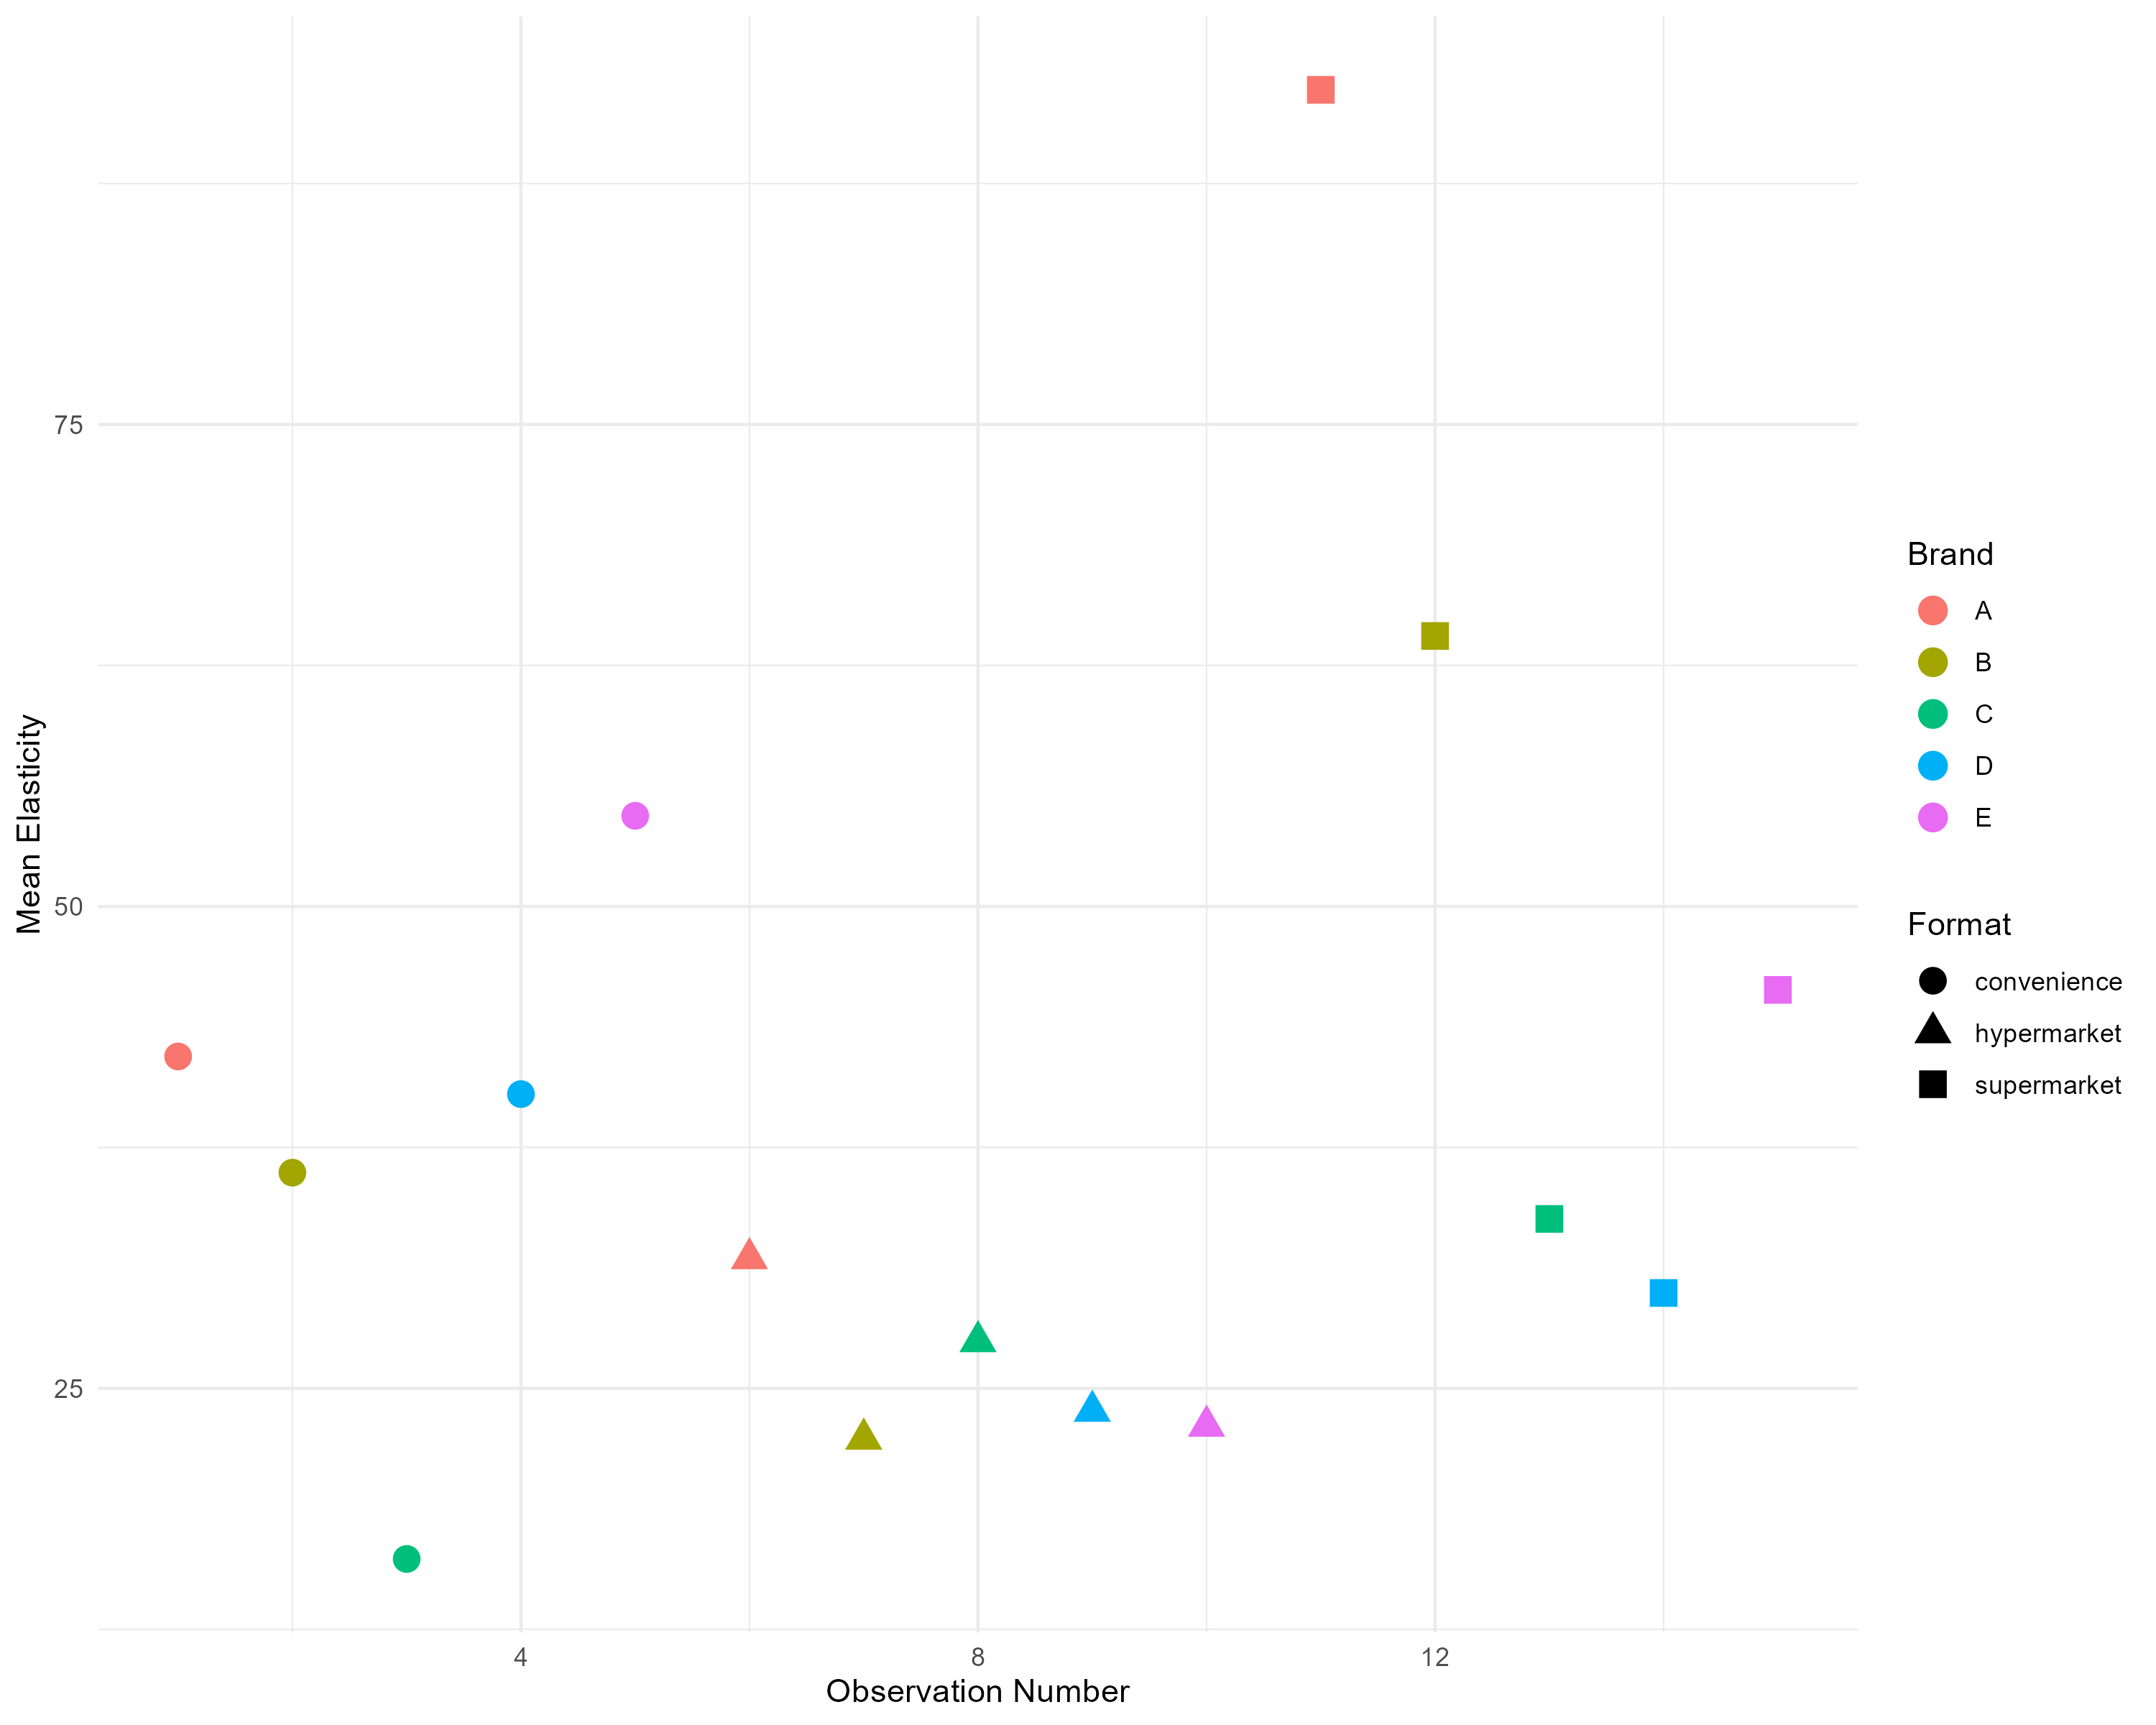
\includegraphics{../../gen/firststage/plot_mean_elasticity.png}

\newpage
\section{Second-Stage Analysis}

To see how brand factors, category factors and store formats influence
discount effectiveness, we estimate discounts elasticities at mean
\(\eta_{i,j,k}\) with respect to brand factors, category factors and
store formats. The model for discount elasticity of brand i in category
j in store format k is: \begin{align*}
    \eta_{i,j,k} =\ & \delta_0 + \delta_1 \text{BrandDiscountDepth}_{i,j,k} + \delta_2 \text{BrandDiscountBreadth}_{i,j,k} \nonumber \\
    & + \delta_3 \text{Frequency}_{i,j,k} + \delta_4 \text{PrivateLabel}_{i,j} \nonumber \\
    & + \delta_5 \text{CatDiscountDepth}_{j,k} + \delta_6 \text{CatDiscountBreadth}_{j,k} \nonumber \\
    & + \delta_7 \text{CatDiscProportion}_{j,k} + \delta_8 \text{CatMarketComp}_{j,k} \nonumber \\
    & + \delta_9 \text{Format}_{k}
\end{align*}

The estimate result from aforementioned regression is:

\begin{verbatim}
## 
## Call:
## lm(formula = meanelasticity ~ format + avgbranddiscountdepth + 
##     avgbranddiscountbreath + log(frequency) + PL, data = df, 
##     weights = (1/sdelasticity))
## 
## Weighted Residuals:
##     Min      1Q  Median      3Q     Max 
## -6.4364 -1.9439 -0.4212  2.7380  6.2442 
## 
## Coefficients:
##                         Estimate Std. Error t value Pr(>|t|)
## (Intercept)            -222.5172   436.8004  -0.509    0.624
## formathypermarket       -19.1804    12.3323  -1.555    0.158
## formatsupermarket         5.1736    13.3060   0.389    0.708
## avgbranddiscountdepth     5.9182     5.8236   1.016    0.339
## avgbranddiscountbreath    0.5242     2.0421   0.257    0.804
## log(frequency)           27.3394    94.4796   0.289    0.780
## PL1                      -8.5414     8.3549  -1.022    0.337
## 
## Residual standard error: 4.944 on 8 degrees of freedom
## Multiple R-squared:  0.5158, Adjusted R-squared:  0.1527 
## F-statistic:  1.42 on 6 and 8 DF,  p-value: 0.3146
\end{verbatim}

\end{document}
